% Tipo de documento y otras especificaciones
\documentclass[12pt,letterpaper]{article}
% Para escribir tildes y eñes
\usepackage[utf8]{inputenc}
\usepackage[spanish]{babel} 
\usepackage{verbatim}
\usepackage{multirow}
\usepackage{bigstrut}
\renewcommand{\labelitemi}{$\bullet$}
% Para que los títulos de figuras, tablas y otros estén en español
\usepackage{pgfgantt}%gantt
% Cambiar nombre a tablas
\addto\captionsspanish{\renewcommand{\tablename}{Tabla}}		
% Cambiar nombre a lista de tablas
\addto\captionsspanish{\renewcommand{\listtablename}{Índice de tablas}}
% Tamaño del área de escritura de la página
\usepackage{geometry}
\geometry{left=18mm,right=18mm,top=21mm,bottom=21mm}
% Para insertar gráficas
\usepackage{amsmath}      
\usepackage{amsfonts}    
\usepackage{amssymb}
\usepackage{graphicx} 
\DeclareGraphicsExtensions{.png,.jpg,.eps,}
% Para colocar varias figuras
\usepackage{subfigure}
% Para la presentación correcta de unidades
\usepackage{unitsdef}
% Redimensionamiento del espacio entre magnitud y unidad
\renewcommand{\unitvaluesep}{\hspace*{4pt}}
% Para insertar hipervínculos y marcadores
\usepackage[colorlinks=true,urlcolor=blue,linkcolor=black,citecolor=black]{hyperref}
% Para ubicar las tablas y figuras justo después del texto
\usepackage{float}
% Para hacer tablas más estilizadas
\usepackage{booktabs}
\usepackage{multirow}
\usepackage{mcode}
\batchmode
\bibliographystyle{plain}
\pagestyle{plain}
\pagenumbering{arabic}
\usepackage{lastpage}
\usepackage{enumerate}
% Para manejar los encabezados y pies de página
\usepackage{fancyhdr}
\usepackage{setspace} 
% Contenido de los encabezados y pies de pagina
\pagestyle{fancy}
% Encabezado izquierda
\lhead{IE-0217 Estructuras abstractas de datos y algoritmos para ingeniería} 
\chead{}
% Encabezado derecha
\rhead{Proyecto 1}
% Pie de página izquierda
\lfoot{Escuela de Ingeniería Eléctrica} 
\cfoot{\thepage\ de \pageref{LastPage}}
% Pie de página derecha
\rfoot{Universidad de Costa Rica}

% Referencias
\addto\captionsspanish{\def\refname{Bibliografía}}
%\usepackage[nottoc,notlot,notlof]{tocbibind}

% Portada
\title{
Universidad de Costa Rica\\
{\small Facultad de Ingeniería\\
Escuela de Ingeniería Eléctrica\\
IE-0217 Estructuras abstractas de datos y algoritmos para ingeniería\\
II ciclo 2016\\
\vspace*{0.7in}} Proyecto 2\\ Implementación del juego Hex
\vspace*{0.7in}
}
\author{
Dunia Barahona H, B40806\\
Emmanuel Bustos T, B51296\\{\small Grupo 05}\\
Profesor: M. Sc. Ricardo Román Brenes \vspace*{0.7in}
}

\date{\today\vspace*{0.7in}}  	\setcounter{secnumdepth}{5}

%%%%%%%%%%%%%%%%
\usepackage[at]{easylist}
\ListProperties(Style*=,Numbers=a,FinalMark={.})

\Activate
 % Explicit space after @ needed!!!!!
\newcommand{\spobj}{@ }
\newcommand{\goal}{@@ }
\newcommand{\ind}{@@@ }
\Deactivate

\newenvironment{objectives}
{%
\begin{easylist}
}
{
\end{easylist}
}
%%%%%%%%%%%%%%%%

\begin{document}

\spacing{1.5}
\pdfbookmark[1]{Portada}{portada} 	

% Título
\maketitle

% Índice
\newpage
\tableofcontents
\newpage
\listoffigures

\newpage 
\section{Introducción}
\subsection{Contexto y justificación}
Este trabajo, fue realizado para aprender a hacer uso de las diferentes estructuras de datos que pueden ser utilizadas en la programación. A su vez, se quiso incursionar en los temas que respectan a la creación de una interfaz gráfica, para de esta forma adquirir habilidades y destrezas relacionadas a este tema.
Para el proyecto se escogió el juego $Hex$ debido a que este posee características matemáticas y computacionales bastante atractivas para el desarrollo de los conocimientos previamente mencionados. Por último, al ser este un juego, se presta para la creación de una interfaz gráfica, lo cuál lo hace ideal para lo deseado en el proyecto.

\subsection{Objetivo General}
\begin{enumerate}
\item Realizar la implementación del juego \textit{Hex} en el lenguaje de programación C++. 
\end{enumerate}
\subsection{Objetivos específicos}
\begin{enumerate}
\item Analizar y escoger las estructuras de datos adecuadas para la implementación del juego.
\item Analizar la función de tiempo y complejidad del algotitmo implementado.
\item Verificar que el programa cumpla con las reglas del juego.
\item Construir gráficos para el análisis de los resultados obtenidos.
\item Crear una interfaz gráfica para el juego.
\end{enumerate}

\subsection{Metodología}
La metodología utilizada para el desarrollo de este proyecto consistió en 3 etapas fundamentales, las cuales van a ser desarrolladas a continuación.

La primera etapa correspondió a la investigación bibliográfica acerca del juego, sus especificaciones y reglas. Se trabajó en una laptop HP Pavilion con procesador AMD A8 y una memoria de 5 gigas de RAM, con el sistema operativo Debian Jesse. 

En la segunda etapa, utilizando el equipo previamente mencionado, se creó un código para implementar el juego \textit{Hex} en el lenguaje de programación C++. Este código consta de dos clases y un "main", en el cuál se implementan dichas clases. Además, se creó una interfaz gráfica para jugar $Hex$ de una manera más amigable con el usuario y visualmente más atractiva.

Una vez el que el juego estuvo correctamente implementado, se procedió a la tercera etapa, la cuál consistió en verificar el correcto funcionamiento del programa con cosas como por ejemplo que el programa estuviera detectando las condiciones de gane correctamente, basándose en las reglas del juego, que los turnos transcurrieran con normalidad entre otros aspectos

Una ver realizadas estas tres etapas se realizó el análisis de complejidad del algoritmo implementado, y se comparó con los resultados obtenidos de manera experimental en lo que a tiempos de ejecución respecta.

\section{Marco teórico}
\subsection{Reseña del algoritmo}
En 1942, el ingeniero Danés Piet Hein presentó el juego \textit{Hex} en una coferencia para estudiantes del Instituto de Física Teórica en Dinamarca. El juego se volvió muy popular en ese país bajo el nombre de \textit{Polygon}, a pesar de que Hein lo llamó originalmente $CON-TAC-TIX$.

En 1948 John F. Nash, graduado en matemática de la Universidad de Princeton, reinventó este juego de manera independiente, ganó popularidad rápidamente entre los estudiantes de matemática de la universidad y del Instituto para estudios Avanzados. En esta época el juego era llamado \textit{Nash} o \textit{John}.

En 1952 adquirió el nombre con el que se conoce actualmente, \textit{Hex}, cuando una versión de este juego fue lanzada al mercado por la firma de los hermanos Parker (\textit{Parker Brothers, Inc.}).

El juego llamó la atención, en especial en el área de la matemática, tanto así que el matemático Martin Gardner decidió incluir a $Hex$ en su columna de la revista \textit{Scientific American} llamada \textit{Mathematical Games column.}


\subsection{Funcionamiento del algoritmo}
Hex es un juego de reglas sencillas, pero que requiere de grandes habilidades en estrategia para jugarlo de la mejor manera. Los principales aspectos a tener en cuenta son:
\begin{itemize}
\item Se juega en un tablero en forma de rombo compuesto por celdas hexagonales.
\item El tablero clásico es de 11$\times$11 celdas, pero puede ser de cualquier tamaño.
\item Dos jugadores por partida.
\item A cada jugador le corresponde un color de fichas diferente. Por lo general el color de las fichas es negro y blanco o rojo y azul.
\item Si se usan los colores negro y blanco, las fichas negras colocan primero.
\item Si se usan los colores rojo y azul, las fichas rojas colocan primero.
\item Las fichas solo pueden ponerse en celdas vacías.
\item Cada jugador puede colocar únicamente una ficha por turno.
\item Por la naturaleza del juego no hay manera de que se dé un empate.
\end{itemize}

\begin{figure}[H]
\centering
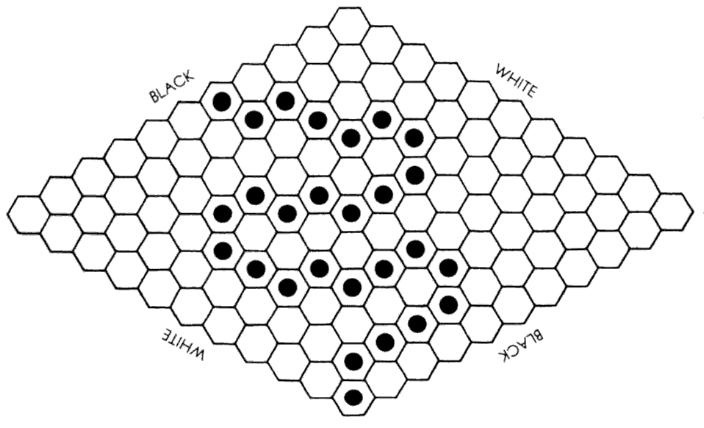
\includegraphics[width=0.7\columnwidth]{tablero.png}
\caption{Cadena ganadora de fichas negras en un tablero $11\times 11$. Tomado de \cite{hexBook}.}
\label{fig:Tablero}
\end{figure}

Al inicio de la partida a cada participante se le asigna un color y dos laterales opuestos del tablero. El objetivo es trazar una línea continua que conecte los extremos del tablero previamente asignados, el jugador que logré esto gana.

\vspace{1 em}

Hex se juega de la siguiente manera:
\begin{itemize}
\item Se rifa a cual participante le corresponde el color rojo y a cual el azul.
\item En este juego el hecho de tener el primer movimiento puede dar una ventaja importante para el desarrollo de la partida, por esta razón después de realizado el primer movimiento, el segundo jugador tiene dos opciones a elegir:
\begin{enumerate}
\item Continuar jugando con las fichas azules.
\item Apropiarse de la jugada hecha por su contrincante y jugar ahora con el color rojo, de esta manera a su adversario le correspondería jugar con las fichas azules.
\end{enumerate}
Sin importar cuál de estas opciones se eligió, el turno siguiente le corresponde al jugador de las fichas azules.\\
Es importante recalcar que esto es válido \textbf{únicamente} después de la primera movida.
\item Los jugadores se turnan para ir colocando fichas, hasta que alguno gane.
\item Se termina el juego.
\end{itemize}

En el programa:
\begin{itemize}
\item Se juega con el color rojo y el color azul.
\item Se ingresa el tamaño del tablero.
\item Se le pedirá al usuario que ingrese las coordenadas correspondientes a la celda donde desea colocar su ficha.
\item Justo después se imprime en la terminal el tablero modificado, con la letra 'R' (rojo) o 'A' (azul) según corresponda, en la posición especificada por el usuario.
\item Se continuarán pidiendo coordenadas hasta que algún jugador gane.
\item Se indica quién ganó y se termina el programa.
\end{itemize}


%Más extensa
\section{Experimentos y análisis de resultados}
\subsection{Experimentos realizados}
%Experimentos que realizará (plataforma, entradas, variables de respuesta, etc.)
Para la realización de los experimentos se hizo uso de diferentes herramientas como la biblioteca de C++ $"time.h"$ con la cuál se obtuvo el tiempo de ejecución de algunos métodos en específico.

En primera instancia, se verificó que el funcionamiento del programa fuera el correcto, tanto el de la interfaz de la consola, como el de la interfaz gráfica, para buscar errores y corregirlos.

Después de comprobar el funcionamiento correcto del programa, se procedió a realizar el análisis correspondiente a tiempo y complejidad del método más importante del programa. El método analizado para la complejidad del programa fue el método $ponroja()$ (el análisis es equivalente para el método $ponazul()$), de la clase $Tablero$. Este método modifica el tablero y verifica constantemente si al realizar ese movimiento el jugador gana la partida o no. Para los experimentos, se muestreó el tiempo de duración de esta función para diferentes tamaños de tablero y se graficaron los resultados.
\subsection{Resultados obtenidos}
Como resultado de este proyecto, se obtuvo un programa en consola completamente funcional, el cuál es completamente interactivo.

Primeramente pregunta las dimensiones deseadas para el tablero, luego pregunta por las coordenadas de la ficha que se desea colocar. Después del primer turno, se aplica la regla del pie, que permite al segundo jugador intercambiar colores con su rival si así lo desea. Se continúan ingresando las coordenadas deseadas para colocar la ficha, además durante cada turno el programa verifica si alguno de los jugadores ha ganado la partida y de ser así lo indica y termina el juego.

\begin{figure}[H]
\centering
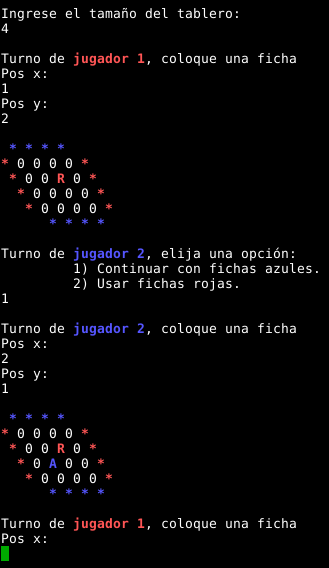
\includegraphics[width=0.5\columnwidth]{main.png}
\caption{Ejecución del programa desde la terminal}
\label{fig:main_1}
\end{figure}

Otro resultado obtenido fue la interfaz gráfica mostrada en la Figura \ref{fig:ig}, la cual hace exactamente lo mismo que el programa de consola, pero con el añadido de que se hace en un entorno gráfico, además de que el jugador no tiene que ingresar las coordenadas en las que desea colocar la ficha en el tablero, sino que directamente puede hacer $click$ en la posición del tablero en la que desea colocar la ficha, la cual se va a teñir del color de la ficha correspondiente al jugador. Cabe destacar que si bien la interfaz funciona correctamente en cuanto a las instrucciones que envía al programa en C++, posee un defecto el cuál no pudo ser corregido a lo largo del proyecto. Dicho defecto consiste en que las fichas se tiñen hasta el turno siguiente, y no cuando el jugador hace $click$ en la posición deseada. 

\begin{figure}[H]
\centering
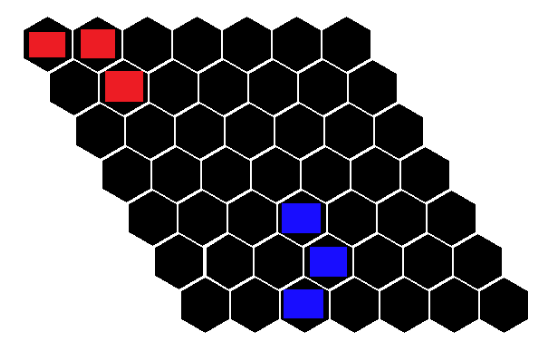
\includegraphics[width=0.6\columnwidth]{ig.png}
\caption{Partida en proceso en la interfaz gráfica}
\label{fig:ig}
\end{figure}



%Pruebas en las q vamos a jugar
%Comprobar q funcione al 100 porciento
%Jugar varias ocasiones y comprobr q sigue las reglas del juego 
%Toda la información se tabuló y se graficó con el fin de comparar los resultados de una forma visual.  
%gráficas cuanto tiempo le toma al programa determinar que hay un ganador


%\subsection{Resultados obtenidos}
%Incluir gráficas
\newpage
\subsection{Análisis de tiempos de ejecución y complejidad computacional}
El análisis correspondiente a la complejidad
Como previamente se mencionó, se estudió el método más importante de todo el programa ($ponroja()$), con el fin de realizar los análisis de tiempo y complejidad de esta, obteniendo los siguentes resultados.
Se obtuvo la siguiente función de tiempo:
\begin{equation}
	3n+32
\end{equation}
A esta función de tiempo se le aplicó la $O$ $grande$  $de$ $Landeau$, de la siguiente manera para obtener la complejidad del método

\begin{equation}
	\mathcal{O}\left(3n+32\right)
\end{equation}
 Finalmente se obtuvo la siguiente complejidad:
\begin{equation}
	n
\end{equation}
la cual corresponde a una complejidad lineal.

Por último, como se mencionó con anterioridad, se graficaron los resultados correspondientes al tiempo de ejecución del programa con respecto a las dimensiones del tablero, obteniendo el siguiente resultado:

\begin{figure}[H]
\centering
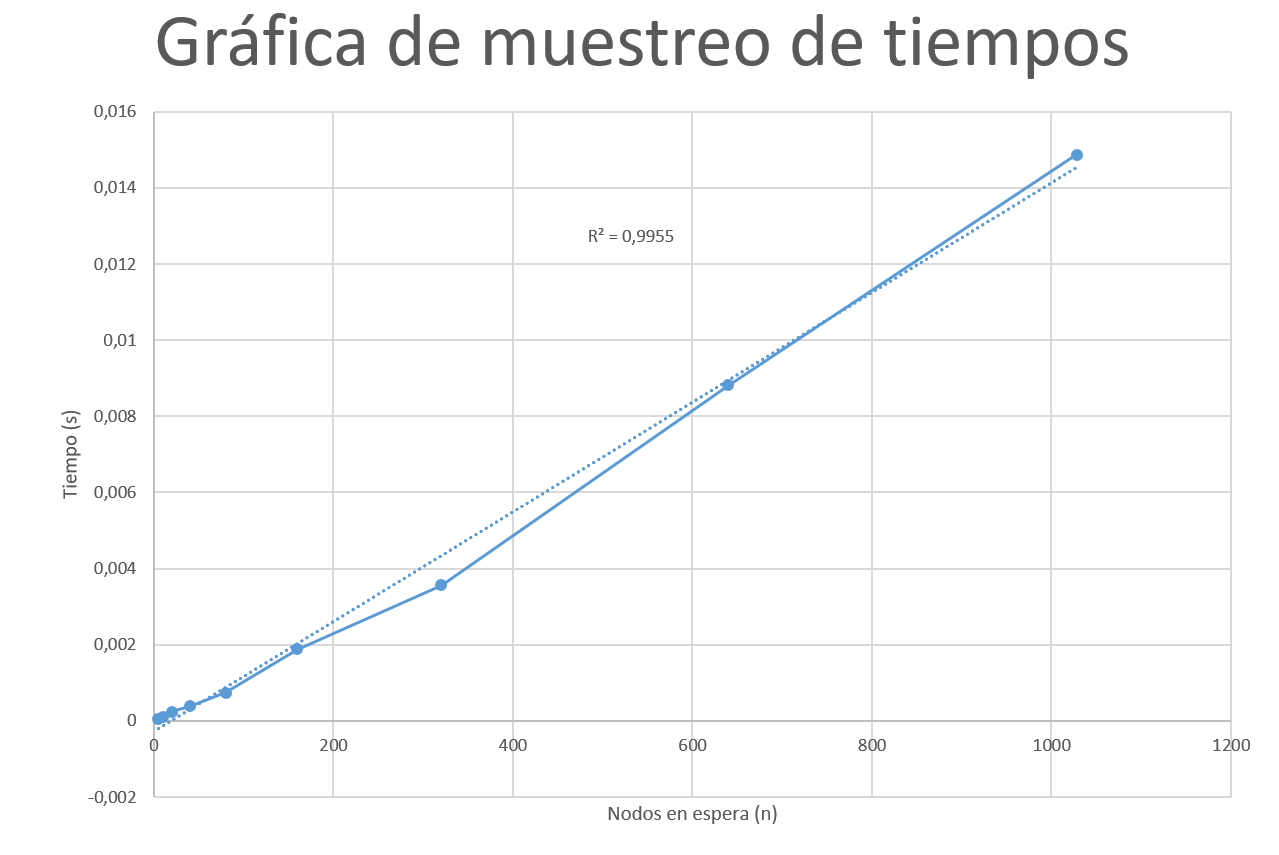
\includegraphics[width=0.6\columnwidth]{g1.png}
\caption{Gráfica de tiempos de ejecución}
\label{fig:graf_1}
\end{figure}

La cual claramente corresponde a una gráfica lineal, con un valor de $R$ lineal muy cercano a 1, lo que confirma el comportamiento lineal del programa, tal y como lo predice el análisis de complejidad previamente realizado.
%Realizando el análisis de tiempo y complejidad pertinente al código se obtuvieron los siguientes resultados:\\
%\indent Función de tiempo:
%\begin{equation}
	%T \left(\right) 
%\end{equation}

%\indent Complejidad
%\begin{equation}
	%\mathcal{O}\left(n\right)
%\end{equation}

%\section{Conclusiones}
%\begin{enumerate}
%\item 
%\end{enumerate}
\section{Conclusiones}
\begin{enumerate}
\item La selección de estructuras de datos adecuadas se una parte fundamental en la creación de un programa, ya que dependiendo de dichas estructuras de datos, el programa funcionará o no de buena forma.

\item Algunas cosas como juegos de mesa que en la vida cotidiana aparentan ser simples, se pueden tornar considerablemente complicadas computacionalmente, como es el caso del $Hex$.

\item La complejidad de un programa puede variar según la implementación de este. Dependiendo de si se utilizan las herramientas y los recursos adecuados a la hora de la creación de un programa, se puede obtener una mejor o peor complejidad.
\end{enumerate}

\addcontentsline{toc}{section}{Bibliografía}
\begin{thebibliography}{1}
\bibitem{hexWeb} Gale, D. (2007). \textit{The Game of Hex and the Brouwer Fixed-Point Theorem}. The American Mathematical Monthly, Vol. 86, No. 10. (Dec., 1979), pp. 818-827. Recuperado el 2 de Noviembre de 2016, de http://www.math.pitt.edu/\~gartside/hex\_Browuer.pdf

\bibitem{hexBook} Gardner, M. (1988). \textit{Hexaflexagons and other Mathematical Diversions. The First Scientific American Book of Mathemathical Puzzles and Games.} USA: The University of Chicago Press.\\Recuperado el 29 de Noviembre de 2016, de https://books.google.co.cr/books?id=QpPlxwSa8akC\\\&printsec=frontcover\&dq=The+Scientific+American+Book+of+Mathematical+Puzzles+and+\\Diversions\&hl=es\&sa=X\&redir\_esc=y\#v=onepage\&q\&f=true

\end{thebibliography}

% http://www.math.pitt.edu/~gartside/hex_Browuer.pdf

% https://books.google.co.cr/books?id=QpPlxwSa8akC&printsec=frontcover&dq=The+Scientific+American+Book+of+Mathematical+Puzzles+and+Diversions&hl=es&sa=X&redir_esc=y#v=onepage&q=hex%20game&f=false
\newpage

\section{Anexos}
\subsection{Main}
\subsubsection*{main.cpp}
\begin{lstlisting}
#include "Tablero.h"
#include "Ficha.h"

using namespace std;
int main(int argc, char** argv) {
	//Variables utilizadas durante el juego
	int a= -1; 
	int b= -1;
	int opc= 0; //option
	int tab;
	bool turno; //Booleano que indica si el turno de un jugador esta activo 
	
	cout<<endl<<"Ingrese las dimensiones del tablero:"<<endl;
	cin>>tab;
	Tablero t(tab); //Se inicializa el tablero
	
	cout<<endl<<"Turno de";
	printf("%c[%d;%dm jugador 1%c[%dm",27,1,31,27,0);
	cout<<", coloque una ficha"<<endl;

    while ( (a<0 || a>=tab) || (b<0 || b>=tab) ) {
		cout<<"Pos x:"<<endl; //Posiciones "x" y "y" de las ficha deseada.
		cin>>a; 
		cout<<"Pos y:"<<endl;
		cin>>b;			
		if ( (a<0 || a>=tab) || (b<0 || b>=tab) ) {
			cout<<"Posicion fuera del tablero."<<endl<<endl;
		}
	}
	
	turno=t.ponroja(a,b);
	cout<<endl;
	~t;    
	while (opc!=1 && opc!=2) {
		cout<<endl<<"Turno de";
		printf("%c[%d;%dm jugador 2%c[%dm",27,1,34,27,0);
		cout<<", elija una opcion:"<<endl;
		cout<<"\t 1) Continuar con fichas azules."<<endl<<"\t 2) Usar fichas rojas."<<endl;
		cin>>opc;
		if (opc!=1 && opc!=2) {
			cout<<opc<<"no es una opcion."<<endl;
		}
	}	
	while(t.ganar==false){ //mientras ninguno de los jugadores haya ganado
		turno=false;
		if (opc==1) {
			while(turno!=true){ //turno del jugador azul
				if(t.ganar==true){break;}
				cout<<endl<<"Turno de";
				printf("%c[%d;%dm jugador 2%c[%dm",27,1,34,27,0);
				cout<<", coloque una ficha"<<endl;
				
				a= -1;
				b= -1;
				while ( (a<0 || a>=tab) || (b<0 || b>=tab) ) {
					cout<<"Pos x:"<<endl;
					cin>>a;	
					cout<<"Pos y:"<<endl;
					cin>>b;
					if ( (a<0 || a>=tab) || (b<0 || b>=tab) ) {
						cout<<"Posicion fuera del tablero."<<endl<<endl;
					}
				} turno=t.ponazul(a,b); //Esto hace que el jugador coloque la ficha
				//Si la ficha colocada por el jugador conecta con el inicio y el final
                del tablero, el jugador gana.
				if(*t.tablero[a][b].conectainicio==true
                && *t.tablero[a][b].conectafinal==true){t.ganar=true;}
				cout<<endl;
				~t; //Imprimir el tablero
			}
			turno=false;
				
			while(turno!=true){ //mientras el turno del jugador este activo, no pasar al
            siguiente turno
            	//Al encontrar ganador, terminar el juego inmediatamente
				if(t.ganar==true){break;}
				cout<<endl<<"Turno de";
				printf("%c[%d;%dm jugador 1%c[%dm",27,1,31,27,0);
				cout<<", coloque una ficha"<<endl;
					
				a= -1;
				b= -1;
				while ( (a<0 || a>=tab) || (b<0 || b>=tab) ) {
					cout<<"Pos x:"<<endl;
					cin>>a;
					cout<<"Pos y:"<<endl;
					cin>>b;
					if ( (a<0 || a>=tab) || (b<0 || b>=tab) ) {
						cout<<"Posicion fuera del tablero."<<endl<<endl;
					}
				}
                turno=t.ponroja(a,b);
				if(*t.tablero[a][b].conectainicio==true &&
                *t.tablero[a][b].conectafinal==true){t.ganar=true;} 
				cout<<endl;
				~t; 
			}
		}	
		else if (opc==2)
		{
			while(turno!=true){ //turno del jugador azul
				if(t.ganar==true){break;}
				cout<<endl<<"Turno de";
				printf("%c[%d;%dm jugador 1%c[%dm",27,1,34,27,0);
				cout<<", coloque una ficha"<<endl;
					
				a= -1;
				b= -1;
				while ( (a<0 || a>=tab) || (b<0 || b>=tab) ) {
					cout<<"Pos x:"<<endl;
					cin>>a;	//Posiciones "x" y "y" de las ficha deseada.
					cout<<"Pos y:"<<endl;
					cin>>b;
						
					if ( (a<0 || a>=tab) || (b<0 || b>=tab) ) {
						cout<<"Posicion fuera del tablero."<<endl<<endl;
					}
				}
                turno=t.ponazul(a,b);
				if(*t.tablero[a][b].conectainicio==true
                && *t.tablero[a][b].conectafinal==true){t.ganar=true;}
				cout<<endl;
				~t;
			}
			turno=false;
				while(turno!=true){ //mientras el turno del jugador este activo
					if(t.ganar==true){break;}
					cout<<endl<<"Turno de";
					printf("%c[%d;%dm jugador 2%c[%dm",27,1,31,27,0);
					cout<<", coloque una ficha"<<endl; 
					
					a= -1;
					b= -1;
					while ( (a<0 || a>=tab) || (b<0 || b>=tab) ) {
						cout<<"Pos x:"<<endl;
						cin>>a;
						cout<<"Pos y:"<<endl;
						cin>>b;
						if ( (a<0 || a>=tab) || (b<0 || b>=tab) ) {
							cout<<endl<<"Posicion fuera del tablero."<<endl<<endl;
						}
					}
                    turno=t.ponroja(a,b); 
					if(*t.tablero[a][b].conectainicio==true
                    && *t.tablero[a][b].conectafinal==true){t.ganar=true;}
					cout<<endl;
					~t;
				}
			}
		}
	// Anunciar Ganador
	if (opc==1)
	{
		cout<<"Partida terminada, el ganador es el";
		if(t.tablero[a][b].rojo==true){
			printf("%c[%d;%dm jugador 1 %c[%dm",27,1,31,27,0);
			cout<<endl;
		}
		else if(t.tablero[a][b].azul==true){
			printf("%c[%d;%dm jugador 2 %c[%dm",27,1,34,27,0);
			cout<<endl;
		}
	}
	else if (opc==2)
	{
		cout<<"Partida terminada, el ganador es el";
		if(t.tablero[a][b].azul==true){
			printf("%c[%d;%dm jugador 1 %c[%dm",27,1,34,27,0);
			cout<<endl;
		}
		else if(t.tablero[a][b].rojo==true){
			printf("%c[%d;%dm jugador 2 %c[%dm",27,1,31,27,0);
			cout<<endl;
		}
	}
	cout<<endl;
	return 0;
}
\end{lstlisting}

\subsection{Clase Ficha}
\subsubsection*{Ficha.h}
\begin{lstlisting}
#ifndef FICHA_H
#define FICHA_H

#include <stdio.h> 
#include <iostream>
#include <list>
#include "string"
#include "stdlib.h"   
#include <cstdlib>
#include <unistd.h>
#include <iostream>
#include "string"
#include <vector>
#include "time.h"

using namespace std;  
class Ficha{
public:
	int* pos;
    bool rojo;
    bool azul;
    bool* conectainicio;
    bool* conectafinal;
    vector<int*> coneci;
    vector<int*> conecf;
	Ficha();	
	~Ficha();
	void operator~();
};
#endif /* FICHA_H */
\end{lstlisting}

\newpage

\subsubsection*{Ficha.cpp}
\begin{lstlisting}
#include "Ficha.h"

Ficha::Ficha(){ // Constructor
	bool* conectai = new bool[1];
	bool* conectaf = new bool[1];
	int* posi= new int[2];
	pos=posi;
	conectainicio=conectai;
	conectafinal=conectaf;
	rojo=false;
	azul=false;
	pos[0]=0;
	pos[1]=0;
	conectainicio[0]=false;
	conectafinal[0]=false;
}

Ficha::~Ficha(){
}

void Ficha::operator~(){ // Imprimir ficha
	cout<<"Color de ficha: "; 
	if(this->rojo){cout<<"Rojo"<<endl;}
	else if(this->azul){cout<<"Azul"<<endl;}
	else{cout<<"Sin color"<< endl;} 
	cout<<"Anclada al inicio: "; 
	if(*conectainicio){cout<<"Si"<<endl;}
	else{cout<<"No"<<endl;}
	cout<<"Anclada al final: ";
	if(*conectafinal){cout<<"Si"<<endl;}
	else{cout<<"No"<<endl;}	
}
\end{lstlisting}

\subsection{Clase Tablero}
\subsubsection*{Tablero.h}
\begin{lstlisting}
#ifndef TABLERO_H
#define TABLERO_H

#include "Ficha.h"

using namespace std;                    
class Tablero{
public:
    Ficha** tablero;
    int size;
    bool ganar;
	Tablero();	
	Tablero(int t);
	bool ponroja(int a, int b);
	bool ponazul(int a, int b);
	~Tablero();
	void operator~();
};
#endif /* TABLERO_H */
\end{lstlisting}

\subsubsection*{Tablero.cpp}
\begin{lstlisting}
#include "Tablero.h"

Tablero::Tablero(){ // Constructor de clase Tablero	
}

Tablero::Tablero(int i){
	this->size=i;
	Ficha** tab = new Ficha*[i];
	for(int j=0; j<i; j++){
		tab[j]=new Ficha[i];
	}
	this->tablero=tab;
}

Tablero::~Tablero(){ // Destructor de la clase Tablero
}

void Tablero::operator~(){ // Imprimir tablero
	int m=1;
	
	//borde superior
	cout<<" ";
	for(int bs=0; bs<size; bs++){
		printf("%c[%d;%dm* %c[%dm",27,1,34,27,0);
	}
	cout<<endl;
    //
	for(int i=0;i<size;i++){
		for(int j=0;j<size;j++){
			if (j==0) //borde derecho {
				printf("%c[%d;%dm* %c[%dm",27,1,31,27,0);	
			}
			if(tablero[i][j].rojo) {
				printf("%c[%d;%dmR %c[%dm",27,1,31,27,0);
			}
			if(tablero[i][j].azul) {
				printf("%c[%d;%dmA %c[%dm",27,1,34,27,0);
			}
			else if(tablero[i][j].rojo==false && tablero[i][j].azul==false){cout<<"0 ";}
			if (j==size-1){ //borde izquierdo
				printf("%c[%d;%dm*%c[%dm",27,1,31,27,0);
			}	
		}	
		cout<<endl;
		for(int k=0; k<m; k++){
		cout<<" ";}
		m++;
	}
	// borde inferior
	cout<<"  ";
	for(int bi=0; bi<size; bi++) {
		printf("%c[%d;%dm* %c[%dm",27,1,34,27,0);
	} 
	cout<<endl;
}
	
// Coloca una ficha roja en el tablero y busca si existe camino posible hasta el inicio
o hasta el final del tablero, verificando el gane.
bool Tablero::ponroja(int a, int b){
	if(tablero[a][b].azul==false){
		tablero[a][b].rojo=true;
		tablero[a][b].pos[0]=a;
		tablero[a][b].pos[1]=b;
		tablero[a][b].coneci.push_back(tablero[a][b].pos);
		tablero[a][b].conecf.push_back(tablero[a][b].pos);
		
        if(b==0) { //verificacion de conexion con inicio
			*tablero[a][b].conectainicio=true;
			if(a!=0 && tablero[a-1][b+1].rojo==true){
				*tablero[a-1][b+1].conectainicio = true;
				for(int i=0; i<tablero[a-1][b+1].coneci.size();i++) {
                	tablero[a][b].coneci.push_back(tablero[a-1][b+1].coneci[i]);
                }
			}
			if(tablero[a][b+1].rojo==true){
				*tablero[a][b+1].conectainicio = true;
				for(int i=0; i<tablero[a][b+1].coneci.size();i++) {
                  tablero[a][b].coneci.push_back(tablero[a][b+1].coneci[i]);
                }
			}
			if(a!=0 && tablero[a-1][b+1].rojo==true &&
            *tablero[a-1][b+1].conectafinal==true){
				*tablero[a][b].conectafinal = true;
			}
			if(tablero[a][b+1].rojo==true && *tablero[a][b+1].conectafinal==true){
				*tablero[a][b].conectafinal = true;
			}
			if(tablero[a][b+1].rojo==true){
				*tablero[a][b+1].conectainicio = true;
				for(int i=0; i<tablero[a][b+1].coneci.size();i++){
					tablero[a][b].coneci.push_back(tablero[a][b+1].coneci[i]);
				}
			}
			if(tablero[a][b+1].rojo==true && *tablero[a][b+1].conectafinal==false){
            	for(int i=0; i<tablero[a][b+1].conecf.size();i++){
            		tablero[a][b].conecf.push_back(tablero[a][b+1].conecf[i]);
				}
				for(int i=0; i<tablero[a][b].conecf.size();i++){
                	tablero[tablero[a][b].conecf[i][0]]
                    [tablero[a][b].coneci[i][1]].conecf=tablero[a][b].conecf;
				}
			}
			if(a!=0 && tablero[a-1][b+1].rojo==true &&
            *tablero[a-1][b+1].conectafinal==false){
            	for(int i=0; i<tablero[a-1][b+1].conecf.size();i++){
                		tablero[a][b].conecf.push_back(tablero[a-1][b+1].conecf[i]);
				}
				for(int i=0; i<tablero[a][b].conecf.size();i++){
                	tablero[tablero[a][b].conecf[i][0]]
                    [tablero[a][b].conecf[i][1]].conecf=tablero[a][b].conecf;
				}
			}
		}
		if(b==size-1){	
			if(a!=size-1 && tablero[a+1][b-1].rojo==true){
				for(int i=0; i<tablero[a+1][b-1].coneci.size();i++){
                	tablero[a][b].coneci.push_back(tablero[a+1][b-1].coneci[i]);
				}
			}
			if(tablero[a][b-1].rojo==true){
				for(int i=0; i<tablero[a][b-1].coneci.size();i++){
                	tablero[a][b].coneci.push_back(tablero[a][b-1].coneci[i]);
				}
			}
			if(a!=size-1 && tablero[a+1][b-1].rojo==true
            && *tablero[a+1][b-1].conectafinal==true ){
				*tablero[a][b].conectafinal = true;
			}
			if(tablero[a][b-1].rojo==true && *tablero[a][b-1].conectafinal==true){
				*tablero[a][b].conectafinal = true;
			}
			
			if(tablero[a][b-1].rojo==true){
				for(int i=0; i<tablero[a][b-1].coneci.size();i++){
                	tablero[a][b].coneci.push_back(tablero[a][b-1].coneci[i]);
				}
			}
		}
		else if(b!=0 && b!=size-1){
			if(*tablero[a][b].conectainicio==true){
				if(a!=0 && a!=size-1){
					if(tablero[a-1][b+1].rojo==true){
						for(int i=0; i<tablero[a-1][b+1].coneci.size();i++){
							tablero[a][b].coneci.push_back(tablero[a-1][b+1].coneci[i]);
						}
					}
					if(tablero[a+1][b-1].rojo==true){
						for(int i=0; i<tablero[a+1][b-1].coneci.size();i++){
							tablero[a][b].coneci.push_back(tablero[a+1][b-1].coneci[i]);
						}
					}
					if(tablero[a][b+1].rojo==true){
						for(int i=0; i<tablero[a][b+1].coneci.size();i++){
							tablero[a][b].coneci.push_back(tablero[a][b+1].coneci[i]);
						}
					}
					if(tablero[a][b-1].rojo==true){
						for(int i=0; i<tablero[a][b-1].coneci.size();i++){
							tablero[a][b].coneci.push_back(tablero[a][b-1].coneci[i]);
						}
					}
					if(tablero[a-1][b].rojo==true){
						for(int i=0; i<tablero[a-1][b].coneci.size();i++){
							tablero[a][b].coneci.push_back(tablero[a-1][b].coneci[i]);
						}
					}
					if(tablero[a+1][b].rojo==true){
						for(int i=0; i<tablero[a+1][b].coneci.size();i++){
							tablero[a][b].coneci.push_back(tablero[a+1][b].coneci[i]);
						}
					}
				}
				else if(a==0){
					if(tablero[a+1][b-1].rojo==true){
						for(int i=0; i<tablero[a+1][b-1].coneci.size();i++){
							tablero[a][b].coneci.push_back(tablero[a+1][b-1].coneci[i]);
						}
					}
					if(tablero[a][b+1].rojo==true){
						for(int i=0; i<tablero[a][b+1].coneci.size();i++){
							tablero[a][b].coneci.push_back(tablero[a][b+1].coneci[i]);
						}
					}
					if(tablero[a][b-1].rojo==true){
						for(int i=0; i<tablero[a][b-1].coneci.size();i++){
							tablero[a][b].coneci.push_back(tablero[a][b-1].coneci[i]);
						}
					}
					if(tablero[a+1][b].rojo==true){
						for(int i=0; i<tablero[a+1][b].coneci.size();i++){
							tablero[a][b].coneci.push_back(tablero[a+1][b].coneci[i]);
						}
					}
				}
				else if(a==size-1){
					if(tablero[a-1][b+1].rojo==true){
						for(int i=0; i<tablero[a-1][b+1].coneci.size();i++){
							tablero[a][b].coneci.push_back(tablero[a-1][b+1].coneci[i]);
						}
					}
					if(tablero[a][b+1].rojo==true){
						for(int i=0; i<tablero[a][b+1].coneci.size();i++){
							tablero[a][b].coneci.push_back(tablero[a][b+1].coneci[i]);
						}
					}
					if(tablero[a][b-1].rojo==true){
						for(int i=0; i<tablero[a][b-1].coneci.size();i++){
							tablero[a][b].coneci.push_back(tablero[a][b-1].coneci[i]);
						}
					}
					if(tablero[a-1][b].rojo==true){
						for(int i=0; i<tablero[a-1][b].coneci.size();i++){
							tablero[a][b].coneci.push_back(tablero[a-1][b].coneci[i]);
						}
					}
				}
			}
			else if(*tablero[a][b].conectainicio==false){
				if(a!=0 && a!=size-1){
					if(tablero[a-1][b+1].rojo==true
                    && *tablero[a-1][b+1].conectainicio==false){
						for(int i=0; i<tablero[a-1][b+1].coneci.size();i++){
							tablero[a][b].coneci.push_back(tablero[a-1][b+1].coneci[i]);
						}
						for(int i=0; i<tablero[a][b].coneci.size();i++){
							tablero[tablero[a][b].coneci[i][0]]
                            [tablero[a][b].coneci[i][1]].coneci=tablero[a][b].coneci;
						}
					}
					if(tablero[a+1][b-1].rojo==true
                    && *tablero[a+1][b-1].conectainicio==false){
						for(int i=0; i<tablero[a+1][b-1].coneci.size();i++){
							tablero[a][b].coneci.push_back(tablero[a+1][b-1].coneci[i]);
						}
						for(int i=0; i<tablero[a][b].coneci.size();i++){
							tablero[tablero[a][b].coneci[i][0]]
                            [tablero[a][b].coneci[i][1]].coneci=tablero[a][b].coneci;
						}
					}
					if(tablero[a][b+1].rojo==true && *tablero[a][b+1].conectainicio==false){
						for(int i=0; i<tablero[a][b+1].coneci.size();i++){
							tablero[a][b].coneci.push_back(tablero[a][b+1].coneci[i]);
						}
						for(int i=0; i<tablero[a][b].coneci.size();i++){
							tablero[tablero[a][b].coneci[i][0]]
                            [tablero[a][b].coneci[i][1]].coneci=tablero[a][b].coneci;
						}
					}
					if(tablero[a][b-1].rojo==true && *tablero[a][b-1].conectainicio==false){
						for(int i=0; i<tablero[a][b-1].coneci.size();i++){
							tablero[a][b].coneci.push_back(tablero[a][b-1].coneci[i]);
					}
						for(int i=0; i<tablero[a][b].coneci.size();i++){
							tablero[tablero[a][b].coneci[i][0]]
                            [tablero[a][b].coneci[i][1]].coneci=tablero[a][b].coneci;
						}
					}
					if(tablero[a-1][b].rojo==true && *tablero[a-1][b].conectainicio==false){
						for(int i=0; i<tablero[a-1][b].coneci.size();i++){
							tablero[a][b].coneci.push_back(tablero[a-1][b].coneci[i]);
						}
						for(int i=0; i<tablero[a][b].coneci.size();i++){
							tablero[tablero[a][b].coneci[i][0]]
                            [tablero[a][b].coneci[i][1]].coneci=tablero[a][b].coneci;
						}
					}
					if(tablero[a+1][b].rojo==true && *tablero[a+1][b].conectainicio==false){
						for(int i=0; i<tablero[a+1][b].coneci.size();i++){
							tablero[a][b].coneci.push_back(tablero[a+1][b].coneci[i]);
						}
						for(int i=0; i<tablero[a][b].coneci.size();i++){
							tablero[tablero[a][b].coneci[i][0]]
                            [tablero[a][b].coneci[i][1]].coneci=tablero[a][b].coneci;
						}
					}
				}
				else if(a==0){
					if(tablero[a+1][b-1].rojo==true
                    && *tablero[a+1][b-1].conectainicio==false){
						for(int i=0; i<tablero[a+1][b-1].coneci.size();i++){
							tablero[a][b].coneci.push_back(tablero[a+1][b-1].coneci[i]);
						}
						for(int i=0; i<tablero[a][b].coneci.size();i++){
							tablero[tablero[a][b].coneci[i][0]]
                            [tablero[a][b].coneci[i][1]].coneci=tablero[a][b].coneci;
					}
				}
					if(tablero[a][b+1].rojo==true && *tablero[a][b+1].conectainicio==false){
						for(int i=0; i<tablero[a][b+1].coneci.size();i++){
							tablero[a][b].coneci.push_back(tablero[a][b+1].coneci[i]);
						}
						for(int i=0; i<tablero[a][b].coneci.size();i++){
							tablero[tablero[a][b].coneci[i][0]]
                            [tablero[a][b].coneci[i][1]].coneci=tablero[a][b].coneci;
						}
					}
					if(tablero[a][b-1].rojo==true && *tablero[a][b-1].conectainicio==false){
						for(int i=0; i<tablero[a][b-1].coneci.size();i++){
							tablero[a][b].coneci.push_back(tablero[a][b-1].coneci[i]);
						}
						for(int i=0; i<tablero[a][b].coneci.size();i++){
							tablero[tablero[a][b].coneci[i][0]]
                            [tablero[a][b].coneci[i][1]].coneci=tablero[a][b].coneci;
						}
					}
					if(tablero[a+1][b].rojo==true && *tablero[a+1][b].conectainicio==false){
						for(int i=0; i<tablero[a+1][b].coneci.size();i++){
							tablero[a][b].coneci.push_back(tablero[a+1][b].coneci[i]);
						}
						for(int i=0; i<tablero[a][b].coneci.size();i++){
							tablero[tablero[a][b].coneci[i][0]]
                            [tablero[a][b].coneci[i][1]].coneci=tablero[a][b].coneci;
						}
					}
				}
				else if(a==size-1){
					if(tablero[a-1][b+1].rojo==true
                    && *tablero[a-1][b+1].conectainicio==false){
						for(int i=0; i<tablero[a+1][b-1].coneci.size();i++){
							tablero[a][b].coneci.push_back(tablero[a-1][b+1].coneci[i]);
						}
						for(int i=0; i<tablero[a][b].coneci.size();i++){
							tablero[tablero[a][b].coneci[i][0]]
                            [tablero[a][b].coneci[i][1]].coneci=tablero[a][b].coneci;
						}
					}
					if(tablero[a][b+1].rojo==true && *tablero[a][b+1].conectainicio==false){
						for(int i=0; i<tablero[a][b+1].coneci.size();i++){
							tablero[a][b].coneci.push_back(tablero[a][b+1].coneci[i]);
						}
						for(int i=0; i<tablero[a][b].coneci.size();i++){
							tablero[tablero[a][b].coneci[i][0]]
                            [tablero[a][b].coneci[i][1]].coneci=tablero[a][b].coneci;
						}
					}
					if(tablero[a][b-1].rojo==true && *tablero[a][b-1].conectainicio==false){
						for(int i=0; i<tablero[a][b-1].coneci.size();i++){
							tablero[a][b].coneci.push_back(tablero[a][b-1].coneci[i]);
						}
						for(int i=0; i<tablero[a][b].coneci.size();i++){
							tablero[tablero[a][b].coneci[i][0]]
                            [tablero[a][b].coneci[i][1]].coneci=tablero[a][b].coneci;
						}
					}
					if(tablero[a-1][b].rojo==true && *tablero[a-1][b].conectainicio==false){
						for(int i=0; i<tablero[a-1][b].coneci.size();i++){
							tablero[a][b].coneci.push_back(tablero[a-1][b].coneci[i]);
						}
						for(int i=0; i<tablero[a][b].coneci.size();i++){
							tablero[tablero[a][b].coneci[i][0]]
                            [tablero[a][b].coneci[i][1]].coneci=tablero[a][b].coneci;
						}
					}
				}
				if(a!=0 && a!=size-1){
					if(tablero[a-1][b+1].rojo==true&&*tablero[a-1][b+1].conectainicio==true){
						*tablero[a][b].conectainicio=true;
					}
					if(tablero[a+1][b-1].rojo==true&&*tablero[a+1][b-1].conectainicio==true){
						*tablero[a][b].conectainicio=true;
					}
					if(tablero[a][b+1].rojo==true && *tablero[a][b+1].conectainicio==true){
						*tablero[a][b].conectainicio=true;
					}
					if(tablero[a][b-1].rojo==true && *tablero[a][b-1].conectainicio==true){
						*tablero[a][b].conectainicio = true;
					}
					if(tablero[a-1][b].rojo==true && *tablero[a-1][b].conectainicio==true){
						*tablero[a][b].conectainicio=true;
					}
					if(tablero[a+1][b].rojo==true && *tablero[a+1][b].conectainicio==true){
						*tablero[a][b].conectainicio=true;
					}
				}
				else if(a==0){
					if(tablero[a+1][b-1].rojo==true&&*tablero[a+1][b-1].conectainicio==true){
						*tablero[a][b].conectainicio=true;
					}
					if(tablero[a][b+1].rojo==true && *tablero[a][b+1].conectainicio==true){
						*tablero[a][b].conectainicio=true;
					}
					if(tablero[a][b-1].rojo==true && *tablero[a][b-1].conectainicio==true){
						*tablero[a][b].conectainicio=true;
					}
					if(tablero[a+1][b].rojo==true && *tablero[a+1][b].conectainicio==true){
						*tablero[a][b].conectainicio=true;
					}
				}
				else if(a==size-1){
					if(tablero[a-1][b+1].rojo==true&&*tablero[a-1][b+1].conectainicio==true){
						*tablero[a][b].conectainicio=true;
					}
					if(tablero[a][b+1].rojo==true && *tablero[a][b+1].conectainicio==true){
						*tablero[a][b].conectainicio=true;
					}
					if(tablero[a][b-1].rojo==true && *tablero[a][b-1].conectainicio==true){
						*tablero[a][b].conectainicio=true;
					}
					if(tablero[a-1][b].rojo==true && *tablero[a-1][b].conectainicio==true){
						*tablero[a][b].conectainicio=true;
					}
				}
			}
		}
		if(*tablero[a][b].conectainicio==true){
			while(tablero[a][b].coneci.empty()==false){
				*tablero[tablero[a][b].coneci.back()[0]]
                [tablero[a][b].coneci.back()[1]].conectainicio=true;
				tablero[a][b].coneci.pop_back();
			}
		}
		if(b==size-1){ // Verificacion de conexion con el final
			*tablero[a][b].conectafinal=true;
			if(a!=size-1 && tablero[a+1][b-1].rojo==true){
				*tablero[a+1][b-1].conectafinal = true;
				for(int i=0; i<tablero[a+1][b-1].conecf.size();i++){
                	tablero[a][b].conecf.push_back(tablero[a+1][b-1].conecf[i]);
				}
			}
			if(tablero[a][b-1].rojo==true){
				*tablero[a][b-1].conectafinal = true;
				for(int i=0; i<tablero[a][b-1].conecf.size();i++){
                	tablero[a][b].conecf.push_back(tablero[a][b-1].conecf[i]);
				}
			}
			if(a!=size-1 && tablero[a+1][b-1].rojo==true
            && *tablero[a+1][b-1].conectainicio==true){
				*tablero[a][b].conectainicio=true;
			}
			if(tablero[a][b-1].rojo==true && *tablero[a][b-1].conectainicio==true){
				*tablero[a][b].conectainicio=true;
			}
		}
		else if(b!=size-1 && b!=0){
			if(*tablero[a][b].conectafinal==true){
				if(a!=0 && a!=size-1){
					if(tablero[a-1][b+1].rojo==true){
						for(int i=0; i<tablero[a-1][b+1].conecf.size();i++){
							tablero[a][b].conecf.push_back(tablero[a-1][b+1].conecf[i]);
						}
					}
					if(tablero[a+1][b-1].rojo==true){
						for(int i=0; i<tablero[a+1][b-1].conecf.size();i++){
							tablero[a][b].conecf.push_back(tablero[a+1][b-1].conecf[i]);
						}
					}
					if(tablero[a][b+1].rojo==true){
						for(int i=0; i<tablero[a][b+1].conecf.size();i++){
							tablero[a][b].conecf.push_back(tablero[a][b+1].conecf[i]);
						}
					}
					if(tablero[a][b-1].rojo==true){
						for(int i=0; i<tablero[a][b-1].conecf.size();i++){
							tablero[a][b].conecf.push_back(tablero[a][b-1].conecf[i]);
						}
					}
					if(tablero[a-1][b].rojo==true){
						for(int i=0; i<tablero[a-1][b].conecf.size();i++){
							tablero[a][b].conecf.push_back(tablero[a-1][b].conecf[i]);
						}
					}
					if(tablero[a+1][b].rojo==true){
						for(int i=0; i<tablero[a+1][b].conecf.size();i++){
							tablero[a][b].conecf.push_back(tablero[a+1][b].conecf[i]);
						}
					}
				}
				else if(a==0){
					if(tablero[a+1][b-1].rojo==true){
						for(int i=0; i<tablero[a+1][b-1].conecf.size();i++){
							tablero[a][b].conecf.push_back(tablero[a+1][b-1].conecf[i]);
						}
					}
					if(tablero[a][b+1].rojo==true){
						for(int i=0; i<tablero[a][b+1].conecf.size();i++){
							tablero[a][b].conecf.push_back(tablero[a][b+1].conecf[i]);
						}
					}
					if(tablero[a][b-1].rojo==true){
						for(int i=0; i<tablero[a][b-1].conecf.size();i++){
							tablero[a][b].conecf.push_back(tablero[a][b-1].conecf[i]);
						}
					}
					if(tablero[a+1][b].rojo==true){
						for(int i=0; i<tablero[a+1][b].conecf.size();i++){
							tablero[a][b].conecf.push_back(tablero[a+1][b].conecf[i]);
						}
					}
				}
				else if(a==size-1){
					if(tablero[a-1][b+1].rojo==true){
						for(int i=0; i<tablero[a-1][b+1].conecf.size();i++){
							tablero[a][b].conecf.push_back(tablero[a-1][b+1].conecf[i]);
						}
					}
					if(tablero[a][b+1].rojo==true){
						for(int i=0; i<tablero[a][b+1].conecf.size();i++){
							tablero[a][b].conecf.push_back(tablero[a][b+1].conecf[i]);
						}
					}
					if(tablero[a][b-1].rojo==true){
						for(int i=0; i<tablero[a][b-1].conecf.size();i++){
							tablero[a][b].conecf.push_back(tablero[a][b-1].conecf[i]);
						}
					}
					if(tablero[a-1][b].rojo==true){
						for(int i=0; i<tablero[a-1][b].conecf.size();i++){
							tablero[a][b].conecf.push_back(tablero[a-1][b].conecf[i]);
						}
					}
				}
			}
			else if(*tablero[a][b].conectafinal==false){
				if(a!=0 && a!=size-1){
					if(tablero[a-1][b+1].rojo==true&&*tablero[a-1][b+1].conectafinal==false){
						for(int i=0; i<tablero[a-1][b+1].conecf.size();i++){
							tablero[a][b].conecf.push_back(tablero[a-1][b+1].conecf[i]);
						}
						for(int i=0; i<tablero[a][b].conecf.size();i++){
							tablero[tablero[a][b].conecf[i][0]]
                            [tablero[a][b].conecf[i][1]].conecf=tablero[a][b].conecf;
						}
					}
					if(tablero[a+1][b-1].rojo==true&&*tablero[a+1][b-1].conectafinal==false){
						for(int i=0; i<tablero[a+1][b-1].conecf.size();i++){
							tablero[a][b].conecf.push_back(tablero[a+1][b-1].conecf[i]);
						}
						for(int i=0; i<tablero[a][b].conecf.size();i++){
							tablero[tablero[a][b].conecf[i][0]]
                            [tablero[a][b].conecf[i][1]].conecf=tablero[a][b].conecf;
						}
					}
					if(tablero[a][b+1].rojo==true && *tablero[a][b+1].conectafinal==false){
						for(int i=0; i<tablero[a][b+1].conecf.size();i++){
							tablero[a][b].conecf.push_back(tablero[a][b+1].conecf[i]);
						}
						for(int i=0; i<tablero[a][b].conecf.size();i++){
							tablero[tablero[a][b].conecf[i][0]]
                            [tablero[a][b].conecf[i][1]].conecf=tablero[a][b].conecf;
						}
					}
					if(tablero[a][b-1].rojo==true && *tablero[a][b-1].conectafinal==false){
						for(int i=0; i<tablero[a][b-1].conecf.size();i++){
							tablero[a][b].conecf.push_back(tablero[a][b-1].conecf[i]);
						}
						for(int i=0; i<tablero[a][b].conecf.size();i++){
							tablero[tablero[a][b].conecf[i][0]]
                            [tablero[a][b].conecf[i][1]].conecf=tablero[a][b].conecf;
						}
					}
					if(tablero[a-1][b].rojo==true && *tablero[a-1][b].conectafinal==false){
						for(int i=0; i<tablero[a-1][b].conecf.size();i++){
							tablero[a][b].conecf.push_back(tablero[a-1][b].conecf[i]);
						}
						for(int i=0; i<tablero[a][b].conecf.size();i++){
							tablero[tablero[a][b].conecf[i][0]]
                            [tablero[a][b].conecf[i][1]].conecf=tablero[a][b].conecf;
						}
					}
					if(tablero[a+1][b].rojo==true && *tablero[a+1][b].conectafinal==false){
						for(int i=0; i<tablero[a+1][b].conecf.size();i++){
							tablero[a][b].conecf.push_back(tablero[a+1][b].conecf[i]);
						}
						for(int i=0; i<tablero[a][b].conecf.size();i++){
							tablero[tablero[a][b].conecf[i][0]]
                            [tablero[a][b].conecf[i][1]].conecf=tablero[a][b].conecf;
						}
					}
				}
				else if(a==0){
					if(tablero[a+1][b-1].rojo==true&&*tablero[a+1][b-1].conectafinal==false){
						for(int i=0; i<tablero[a+1][b-1].conecf.size();i++){
							tablero[a][b].conecf.push_back(tablero[a+1][b-1].conecf[i]);
						}
						for(int i=0; i<tablero[a][b].conecf.size();i++){
							tablero[tablero[a][b].conecf[i][0]]
                            [tablero[a][b].conecf[i][1]].conecf=tablero[a][b].conecf;
						}
					}
					if(tablero[a][b+1].rojo==true && *tablero[a][b+1].conectafinal==false){
						for(int i=0; i<tablero[a][b+1].conecf.size();i++){
							tablero[a][b].conecf.push_back(tablero[a][b+1].conecf[i]);
						}
						for(int i=0; i<tablero[a][b].conecf.size();i++){
							tablero[tablero[a][b].conecf[i][0]]
                            [tablero[a][b].conecf[i][1]].conecf=tablero[a][b].conecf;
						}
					}
					if(tablero[a][b-1].rojo==true && *tablero[a][b-1].conectafinal==false){
						for(int i=0; i<tablero[a][b-1].conecf.size();i++){
							tablero[a][b].conecf.push_back(tablero[a][b-1].conecf[i]);
						}
						for(int i=0; i<tablero[a][b].conecf.size();i++){
							tablero[tablero[a][b].conecf[i][0]]
                            [tablero[a][b].conecf[i][1]].conecf=tablero[a][b].conecf;
						}
					}
					if(tablero[a+1][b].rojo==true && *tablero[a+1][b].conectafinal==false){
						for(int i=0; i<tablero[a+1][b].conecf.size();i++){
							tablero[a][b].conecf.push_back(tablero[a+1][b].conecf[i]);
						}
						for(int i=0; i<tablero[a][b].conecf.size();i++){
							tablero[tablero[a][b].conecf[i][0]]
                            [tablero[a][b].conecf[i][1]].conecf=tablero[a][b].conecf;
						}
					}
				}
				else if(a==size-1){
					if(tablero[a-1][b+1].rojo==true&&*tablero[a-1][b+1].conectafinal==false){
						for(int i=0; i<tablero[a-1][b+1].conecf.size();i++){
							tablero[a][b].conecf.push_back(tablero[a-1][b+1].conecf[i]);
						}
						for(int i=0; i<tablero[a][b].conecf.size();i++){
							tablero[tablero[a][b].conecf[i][0]]
                            [tablero[a][b].conecf[i][1]].conecf=tablero[a][b].conecf;
						}
					}
					if(tablero[a][b+1].rojo==true && *tablero[a][b+1].conectafinal==false){
						for(int i=0; i<tablero[a][b+1].conecf.size();i++){
							tablero[a][b].conecf.push_back(tablero[a][b+1].conecf[i]);
						}
						for(int i=0; i<tablero[a][b].conecf.size();i++){
							tablero[tablero[a][b].conecf[i][0]]
                            [tablero[a][b].conecf[i][1]].conecf=tablero[a][b].conecf;
						}
					}
					if(tablero[a][b-1].rojo==true && *tablero[a][b-1].conectafinal==false){
						for(int i=0; i<tablero[a][b-1].conecf.size();i++){
							tablero[a][b].conecf.push_back(tablero[a][b-1].conecf[i]);
						}
						for(int i=0; i<tablero[a][b].conecf.size();i++){
							tablero[tablero[a][b].conecf[i][0]]
                            [tablero[a][b].conecf[i][1]].conecf=tablero[a][b].conecf;
						}
					}
					if(tablero[a-1][b].rojo==true && *tablero[a-1][b].conectafinal==false){
						for(int i=0; i<tablero[a-1][b].conecf.size();i++){
							tablero[a][b].conecf.push_back(tablero[a-1][b].conecf[i]);
						}
						for(int i=0; i<tablero[a][b].conecf.size();i++){
							tablero[tablero[a][b].conecf[i][0]]
                            [tablero[a][b].conecf[i][1]].conecf=tablero[a][b].conecf;
						}
					}
				}
				if(a!=0 && a!=size-1){
					if(tablero[a-1][b+1].rojo==true&&*tablero[a-1][b+1].conectafinal==true){
						*tablero[a][b].conectafinal=true;
					}
					if(tablero[a+1][b-1].rojo==true&&*tablero[a+1][b-1].conectafinal==true){
						*tablero[a][b].conectafinal=true;
					}
					if(tablero[a][b+1].rojo==true && *tablero[a][b+1].conectafinal==true){
						*tablero[a][b].conectafinal=true;
					}
					if(tablero[a][b-1].rojo==true && *tablero[a][b-1].conectafinal==true){
						*tablero[a][b].conectafinal = true;
					}
					if(tablero[a-1][b].rojo==true && *tablero[a-1][b].conectafinal==true){
						*tablero[a][b].conectafinal=true;
					}
					if(tablero[a+1][b].rojo==true && *tablero[a+1][b].conectafinal==true){
						*tablero[a][b].conectafinal=true;
					}
				}
				else if(a==0){
					if(tablero[a+1][b-1].rojo==true&&*tablero[a+1][b-1].conectafinal==true){
						*tablero[a][b].conectafinal=true;
					}
					if(tablero[a][b+1].rojo==true && *tablero[a][b+1].conectafinal==true){
						*tablero[a][b].conectafinal=true;
					}
					if(tablero[a][b-1].rojo==true && *tablero[a][b-1].conectafinal==true){
						*tablero[a][b].conectafinal=true;
					}
					if(tablero[a+1][b].rojo==true && *tablero[a+1][b].conectafinal==true){
						*tablero[a][b].conectafinal=true;
					}
				}
				else if(a==size-1){
					if(tablero[a-1][b+1].rojo==true&&*tablero[a-1][b+1].conectafinal==true){
						*tablero[a][b].conectafinal=true;
					}
					if(tablero[a][b+1].rojo==true && *tablero[a][b+1].conectafinal==true){
						*tablero[a][b].conectafinal=true;
					}
					if(tablero[a][b-1].rojo==true && *tablero[a][b-1].conectafinal==true){
						*tablero[a][b].conectafinal=true;
					}
					if(tablero[a-1][b].rojo==true && *tablero[a-1][b].conectafinal==true){
						*tablero[a][b].conectafinal=true;
					}
				}
			}
		}
		if(*tablero[a][b].conectafinal==true){
			while(tablero[a][b].conecf.empty()==false){
				*tablero[tablero[a][b].conecf.back()[0]]
                [tablero[a][b].conecf.back()[1]].conectafinal=true;
				tablero[a][b].conecf.pop_back();
			}
		}
		return 1;
	}
	else if(tablero[a][b].azul==true){
		cout<<endl<<"Movimiento invalido"<< endl;
		return 0;
	}
}   
// Coloca una ficha azul en el tablero y busca si existe camino posible hasta el inicio
o hasta el final del tablero, verificando el gane.
bool Tablero::ponazul(int a, int b){
	if(tablero[a][b].rojo==false){
		tablero[a][b].azul=true;
		tablero[a][b].pos[0]=a;
		tablero[a][b].pos[1]=b;
		tablero[a][b].coneci.push_back(tablero[a][b].pos);
		tablero[a][b].conecf.push_back(tablero[a][b].pos);
		
		if(a==0){ //verificacion de conexion con inicio
			*tablero[a][b].conectainicio=true;
			if(b!=0 && tablero[a+1][b-1].azul==true){
				*tablero[a+1][b-1].conectainicio = true;
				for(int i=0; i<tablero[a+1][b-1].coneci.size();i++){
                	tablero[a][b].coneci.push_back(tablero[a+1][b-1].coneci[i]);
				}
			}
			if(tablero[a+1][b].azul==true){
				*tablero[a+1][b].conectainicio = true;
				for(int i=0; i<tablero[a+1][b].coneci.size();i++){
                	tablero[a][b].coneci.push_back(tablero[a+1][b].coneci[i]);
				}
			}
			if(b!=0 && tablero[a+1][b-1].azul==true&&*tablero[a+1][b-1].conectafinal==true){
				*tablero[a][b].conectafinal = true;
			}
			if(tablero[a+1][b].azul==true && *tablero[a+1][b].conectafinal==true){
				*tablero[a][b].conectafinal = true;
			}
			if(tablero[a+1][b].azul==true && *tablero[a+1][b].conectafinal==false){
            	for(int i=0; i<tablero[a+1][b].conecf.size();i++){
                	tablero[a][b].conecf.push_back(tablero[a+1][b].conecf[i]);
				}
				for(int i=0; i<tablero[a][b].conecf.size();i++){
                	tablero[tablero[a][b].conecf[i][0]]
                    [tablero[a][b].coneci[i][1]].conecf=tablero[a][b].conecf;
				}
			}
			if(b!=0 && tablero[a+1][b-1].azul==true&&*tablero[a+1][b-1].conectafinal==false){
            	for(int i=0; i<tablero[a+1][b-1].conecf.size();i++){
                	tablero[a][b].conecf.push_back(tablero[a+1][b-1].conecf[i]);
				}
                for(int i=0; i<tablero[a][b].conecf.size();i++){
                	tablero[tablero[a][b].conecf[i][0]]
                    [tablero[a][b].conecf[i][1]].conecf=tablero[a][b].conecf;
				}
			}
		}	
		if(a==size-1){	
			if(b!=size-1 && tablero[a-1][b+1].azul==true){
				for(int i=0; i<tablero[a-1][b+1].coneci.size();i++){
                	tablero[a][b].coneci.push_back(tablero[a-1][b+1].coneci[i]);
				}
			} 
			if(tablero[a-1][b].azul==true){
				for(int i=0; i<tablero[a-1][b].coneci.size();i++){
                	tablero[a][b].coneci.push_back(tablero[a-1][b].coneci[i]);
				}
			}
			if(b!=size-1 && tablero[a-1][b+1].azul==true
            && *tablero[a-1][b+1].conectainicio==true){
				*tablero[a][b].conectainicio=true;
			}
			if(tablero[a-1][b].azul==true && *tablero[a-1][b].conectainicio==true){
				*tablero[a][b].conectainicio=true;
			}
			if(b!=size-1 && tablero[a-1][b+1].azul==true
            && *tablero[a-1][b+1].conectafinal==true ){
				*tablero[a][b].conectafinal = true;
			}
			if(tablero[a-1][b].azul==true && *tablero[a-1][b].conectafinal==true){
				*tablero[a][b].conectafinal = true;
			}
			if(tablero[a-1][b].azul==true){
				for(int i=0; i<tablero[a-1][b].coneci.size();i++){
                	tablero[a][b].coneci.push_back(tablero[a-1][b].coneci[i]);
				}
			}
		} 
		else if(a!=0 && a!=size-1){
			if(*tablero[a][b].conectainicio==true){
				if(b!=0 && b!=size-1){
					if(tablero[a-1][b+1].azul==true){
						for(int i=0; i<tablero[a-1][b+1].coneci.size();i++){
							tablero[a][b].coneci.push_back(tablero[a-1][b+1].coneci[i]);
						}
					}
					if(tablero[a+1][b-1].azul==true){
						for(int i=0; i<tablero[a+1][b-1].coneci.size();i++){
							tablero[a][b].coneci.push_back(tablero[a+1][b-1].coneci[i]);
						}
					}
					if(tablero[a][b+1].azul==true){
						for(int i=0; i<tablero[a][b+1].coneci.size();i++){
							tablero[a][b].coneci.push_back(tablero[a][b+1].coneci[i]);
						}
					}
					if(tablero[a][b-1].azul==true){
						for(int i=0; i<tablero[a][b-1].coneci.size();i++){
							tablero[a][b].coneci.push_back(tablero[a][b-1].coneci[i]);
						}
					}
					if(tablero[a-1][b].azul==true){
						for(int i=0; i<tablero[a-1][b].coneci.size();i++){
							tablero[a][b].coneci.push_back(tablero[a-1][b].coneci[i]);
						}
					}
					if(tablero[a+1][b].azul==true){
						for(int i=0; i<tablero[a+1][b].coneci.size();i++){
							tablero[a][b].coneci.push_back(tablero[a+1][b].coneci[i]);
						}
					}
				}
				else if(b==0){
					if(tablero[a-1][b+1].azul==true){
						for(int i=0; i<tablero[a-1][b+1].coneci.size();i++){
							tablero[a][b].coneci.push_back(tablero[a-1][b+1].coneci[i]);
						}
					}
					if(tablero[a+1][b].azul==true){
						for(int i=0; i<tablero[a+1][b].coneci.size();i++){
							tablero[a][b].coneci.push_back(tablero[a+1][b].coneci[i]);
						}
					}
					if(tablero[a-1][b].azul==true){
						for(int i=0; i<tablero[a-1][b].coneci.size();i++){
							tablero[a][b].coneci.push_back(tablero[a-1][b].coneci[i]);
						}
					}
					if(tablero[a][b+1].azul==true){
						for(int i=0; i<tablero[a][b+1].coneci.size();i++){
							tablero[a][b].coneci.push_back(tablero[a][b+1].coneci[i]);
						}
					}
				}
				else if(b==size-1){
					if(tablero[a+1][b-1].azul==true){
						for(int i=0; i<tablero[a+1][b-1].coneci.size();i++){
							tablero[a][b].coneci.push_back(tablero[a+1][b-1].coneci[i]);
						}
					}
					if(tablero[a-1][b].azul==true){
						for(int i=0; i<tablero[a-1][b].coneci.size();i++){
							tablero[a][b].coneci.push_back(tablero[a-1][b].coneci[i]);
						}
					}
					if(tablero[a+1][b].azul==true){
						for(int i=0; i<tablero[a+1][b].coneci.size();i++){
							tablero[a][b].coneci.push_back(tablero[a+1][b].coneci[i]);
						}
					}
					if(tablero[a][b-1].azul==true){
						for(int i=0; i<tablero[a][b-1].coneci.size();i++){
							tablero[a][b].coneci.push_back(tablero[a][b-1].coneci[i]);
						}
					}
				}
			}
			else if(*tablero[a][b].conectainicio==false){
				if(b!=0 && b!=size-1){
					if(tablero[a-1][b+1].azul==true
                    && *tablero[a-1][b+1].conectainicio==false){
						for(int i=0; i<tablero[a-1][b+1].coneci.size();i++){
							tablero[a][b].coneci.push_back(tablero[a-1][b+1].coneci[i]);
						}
						for(int i=0; i<tablero[a][b].coneci.size();i++){
							tablero[tablero[a][b].coneci[i][0]]
                            [tablero[a][b].coneci[i][1]].coneci=tablero[a][b].coneci;
						}
					}
					if(tablero[a+1][b-1].azul==true
                    && *tablero[a+1][b-1].conectainicio==false){
						for(int i=0; i<tablero[a+1][b-1].coneci.size();i++){
							tablero[a][b].coneci.push_back(tablero[a+1][b-1].coneci[i]);
						}
						for(int i=0; i<tablero[a][b].coneci.size();i++){
							tablero[tablero[a][b].coneci[i][0]]
                            [tablero[a][b].coneci[i][1]].coneci=tablero[a][b].coneci;
						}
					}
					if(tablero[a][b+1].azul==true && *tablero[a][b+1].conectainicio==false){
						for(int i=0; i<tablero[a][b+1].coneci.size();i++){
							tablero[a][b].coneci.push_back(tablero[a][b+1].coneci[i]);
						}
						for(int i=0; i<tablero[a][b].coneci.size();i++){
							tablero[tablero[a][b].coneci[i][0]]
                            [tablero[a][b].coneci[i][1]].coneci=tablero[a][b].coneci;
						}
					}
					if(tablero[a][b-1].azul==true && *tablero[a][b-1].conectainicio==false){
						for(int i=0; i<tablero[a][b-1].coneci.size();i++){
							tablero[a][b].coneci.push_back(tablero[a][b-1].coneci[i]);
						}
						for(int i=0; i<tablero[a][b].coneci.size();i++){
							tablero[tablero[a][b].coneci[i][0]]
                            [tablero[a][b].coneci[i][1]].coneci=tablero[a][b].coneci;
						}
					}
					if(tablero[a-1][b].azul==true && *tablero[a-1][b].conectainicio==false){
						for(int i=0; i<tablero[a-1][b].coneci.size();i++){
							tablero[a][b].coneci.push_back(tablero[a-1][b].coneci[i]);
						}
						for(int i=0; i<tablero[a][b].coneci.size();i++){
							tablero[tablero[a][b].coneci[i][0]]
                            [tablero[a][b].coneci[i][1]].coneci=tablero[a][b].coneci;
						}
					}
					if(tablero[a+1][b].azul==true && *tablero[a+1][b].conectainicio==false){
						for(int i=0; i<tablero[a+1][b].coneci.size();i++){
							tablero[a][b].coneci.push_back(tablero[a+1][b].coneci[i]);
						}
						for(int i=0; i<tablero[a][b].coneci.size();i++){
							tablero[tablero[a][b].coneci[i][0]]
                            [tablero[a][b].coneci[i][1]].coneci=tablero[a][b].coneci;
						}
					}
				}
				else if(b==size-1){
					if(tablero[a+1][b-1].azul==true
                    && *tablero[a+1][b-1].conectainicio==false){
						for(int i=0; i<tablero[a+1][b-1].coneci.size();i++){
							tablero[a][b].coneci.push_back(tablero[a+1][b-1].coneci[i]);
						}
						for(int i=0; i<tablero[a][b].coneci.size();i++){
							tablero[tablero[a][b].coneci[i][0]][tablero[a][b].coneci[i][1]].coneci=tablero[a][b].coneci;
						}
					}
					if(tablero[a-1][b].azul==true && *tablero[a-1][b].conectainicio==false){
						for(int i=0; i<tablero[a-1][b].coneci.size();i++){
							tablero[a][b].coneci.push_back(tablero[a-1][b].coneci[i]);
						}
						for(int i=0; i<tablero[a][b].coneci.size();i++){
							tablero[tablero[a][b].coneci[i][0]]
                            [tablero[a][b].coneci[i][1]].coneci=tablero[a][b].coneci;
						}
					}
					if(tablero[a][b-1].azul==true && *tablero[a][b-1].conectainicio==false){
						for(int i=0; i<tablero[a][b-1].coneci.size();i++){
							tablero[a][b].coneci.push_back(tablero[a][b-1].coneci[i]);
						}
						for(int i=0; i<tablero[a][b].coneci.size();i++){
							tablero[tablero[a][b].coneci[i][0]]
                            [tablero[a][b].coneci[i][1]].coneci=tablero[a][b].coneci;
						}
					}
					if(tablero[a+1][b].azul==true && *tablero[a+1][b].conectainicio==false){
						for(int i=0; i<tablero[a+1][b].coneci.size();i++){
							tablero[a][b].coneci.push_back(tablero[a+1][b].coneci[i]);
						}
						for(int i=0; i<tablero[a][b].coneci.size();i++){
							tablero[tablero[a][b].coneci[i][0]]
                            [tablero[a][b].coneci[i][1]].coneci=tablero[a][b].coneci;
						}
					}
				}
				else if(b==0){
					if(tablero[a-1][b+1].azul==true
                    && *tablero[a-1][b+1].conectainicio==false){
						for(int i=0; i<tablero[a-1][b+1].coneci.size();i++){
							tablero[a][b].coneci.push_back(tablero[a-1][b+1].coneci[i]);
						}
						for(int i=0; i<tablero[a][b].coneci.size();i++){
							tablero[tablero[a][b].coneci[i][0]]
                            [tablero[a][b].coneci[i][1]].coneci=tablero[a][b].coneci;
						}
					}
					if(tablero[a][b+1].azul==true && *tablero[a][b+1].conectainicio==false){
						for(int i=0; i<tablero[a][b+1].coneci.size();i++){
							tablero[a][b].coneci.push_back(tablero[a][b+1].coneci[i]);
						}
						for(int i=0; i<tablero[a][b].coneci.size();i++){
							tablero[tablero[a][b].coneci[i][0]]
                            [tablero[a][b].coneci[i][1]].coneci=tablero[a][b].coneci;
						}
					}
					if(tablero[a+1][b].azul==true && *tablero[a+1][b].conectainicio==false){
						for(int i=0; i<tablero[a+1][b].coneci.size();i++){
							tablero[a][b].coneci.push_back(tablero[a+1][b].coneci[i]);
						}
						for(int i=0; i<tablero[a][b].coneci.size();i++){
							tablero[tablero[a][b].coneci[i][0]]
                            [tablero[a][b].coneci[i][1]].coneci=tablero[a][b].coneci;
						}
					}
					if(tablero[a-1][b].azul==true && *tablero[a-1][b].conectainicio==false){
						for(int i=0; i<tablero[a-1][b].coneci.size();i++){
							tablero[a][b].coneci.push_back(tablero[a-1][b].coneci[i]);
						}
						for(int i=0; i<tablero[a][b].coneci.size();i++){
							tablero[tablero[a][b].coneci[i][0]]
                            [tablero[a][b].coneci[i][1]].coneci=tablero[a][b].coneci;
						}
					}
				}
				if(b!=0 && b!=size-1){
					if(tablero[a-1][b+1].azul==true&&*tablero[a-1][b+1].conectainicio==true){
						*tablero[a][b].conectainicio=true;
					}
					if(tablero[a+1][b-1].azul==tru &&*tablero[a+1][b-1].conectainicio==true){
						*tablero[a][b].conectainicio=true;
					}
					if(tablero[a][b+1].azul==true && *tablero[a][b+1].conectainicio==true){
						*tablero[a][b].conectainicio=true;
					}
					if(tablero[a][b-1].azul==true && *tablero[a][b-1].conectainicio==true){
						*tablero[a][b].conectainicio = true;
					}
					if(tablero[a-1][b].azul==true && *tablero[a-1][b].conectainicio==true){
						*tablero[a][b].conectainicio=true;
					}
					if(tablero[a+1][b].azul==true && *tablero[a+1][b].conectainicio==true){
						*tablero[a][b].conectainicio=true;
					}
				}
				else if(b==size-1){
					if(tablero[a+1][b-1].azul==true&&*tablero[a+1][b-1].conectainicio==true){
						*tablero[a][b].conectainicio=true;
					}
					if(tablero[a+1][b].azul==true && *tablero[a+1][b].conectainicio==true){
						*tablero[a][b].conectainicio=true;
					}
					if(tablero[a][b-1].azul==true && *tablero[a][b-1].conectainicio==true){
						*tablero[a][b].conectainicio=true;
					}
					if(tablero[a-1][b].azul==true && *tablero[a-1][b].conectainicio==true){
						*tablero[a][b].conectainicio=true;
					}
				}
				else if(b==0){
					if(tablero[a-1][b+1].azul==true&&*tablero[a-1][b+1].conectainicio==true){
						*tablero[a][b].conectainicio=true;
					}
					if(tablero[a][b+1].azul==true && *tablero[a][b+1].conectainicio==true){
						*tablero[a][b].conectainicio=true;
					}
					if(tablero[a+1][b].azul==true && *tablero[a+1][b].conectainicio==true){
						*tablero[a][b].conectainicio=true;
					}
					if(tablero[a-1][b].azul==true && *tablero[a-1][b].conectainicio==true){
						*tablero[a][b].conectainicio=true;
					}
				}
			}
		}
		if(*tablero[a][b].conectainicio==true){
			while(tablero[a][b].coneci.empty()==false){
				*tablero[tablero[a][b].coneci.back()[0]]
                [tablero[a][b].coneci.back()[1]].conectainicio=true;
				tablero[a][b].coneci.pop_back();
			}
		}
		if(a==size-1){ //verificacion de conexion con el final
			*tablero[a][b].conectafinal=true;
			if(tablero[a-1][b+1].azul==true){
				*tablero[a-1][b+1].conectafinal = true;
				for(int i=0; i<tablero[a-1][b+1].conecf.size();i++){
                	tablero[a][b].conecf.push_back(tablero[a-1][b+1].conecf[i]);
				}
			}
			if(tablero[a-1][b].azul==true){
				*tablero[a-1][b].conectafinal = true;
				for(int i=0; i<tablero[a-1][b].conecf.size();i++){
                	tablero[a][b].conecf.push_back(tablero[a-1][b].conecf[i]);
				}
			}
			if(tablero[a-1][b+1].azul==true && *tablero[a-1][b+1].conectainicio==true){
				*tablero[a][b].conectainicio=true;
			}
			if(tablero[a-1][b].azul==true && *tablero[a-1][b].conectainicio==true){
				*tablero[a][b].conectainicio=true;
			}
		}
		else if(a!=size-1 && a!=0){
			if(*tablero[a][b].conectafinal==true){
				if(b!=0 && b!=size-1){
					if(tablero[a-1][b+1].azul==true){
						for(int i=0; i<tablero[a-1][b+1].conecf.size();i++){
							tablero[a][b].conecf.push_back(tablero[a-1][b+1].conecf[i]);
						}
					}
					if(tablero[a+1][b-1].azul==true){
						for(int i=0; i<tablero[a+1][b-1].conecf.size();i++){
							tablero[a][b].conecf.push_back(tablero[a+1][b-1].conecf[i]);
						}
					}
					if(tablero[a][b+1].azul==true){
						for(int i=0; i<tablero[a][b+1].conecf.size();i++){
							tablero[a][b].conecf.push_back(tablero[a][b+1].conecf[i]);
						}
					}
					if(tablero[a][b-1].azul==true){
						for(int i=0; i<tablero[a][b-1].conecf.size();i++){
							tablero[a][b].conecf.push_back(tablero[a][b-1].conecf[i]);
						}
					}
					if(tablero[a-1][b].azul==true){
						for(int i=0; i<tablero[a-1][b].conecf.size();i++){
							tablero[a][b].conecf.push_back(tablero[a-1][b].conecf[i]);
						}
					}
					if(tablero[a+1][b].azul==true){
						for(int i=0; i<tablero[a+1][b].conecf.size();i++){
							tablero[a][b].conecf.push_back(tablero[a+1][b].conecf[i]);
						}
					}
				}
				else if(b==0){
					if(tablero[a-1][b+1].azul==true){
						for(int i=0; i<tablero[a-1][b+1].conecf.size();i++){
							tablero[a][b].conecf.push_back(tablero[a-1][b+1].conecf[i]);
						}
					}
					if(tablero[a][b+1].azul==true){
						for(int i=0; i<tablero[a][b+1].conecf.size();i++){
							tablero[a][b].conecf.push_back(tablero[a][b+1].conecf[i]);
						}
					}
					if(tablero[a-1][b].azul==true){
						for(int i=0; i<tablero[a-1][b].conecf.size();i++){
							tablero[a][b].conecf.push_back(tablero[a-1][b].conecf[i]);
						}
					}
					if(tablero[a+1][b].azul==true){
						for(int i=0; i<tablero[a+1][b].conecf.size();i++){
							tablero[a][b].conecf.push_back(tablero[a+1][b].conecf[i]);
						}
					}
				}
				else if(b==size-1){
					if(tablero[a+1][b-1].azul==true){
						for(int i=0; i<tablero[a+1][b-1].conecf.size();i++){
							tablero[a][b].conecf.push_back(tablero[a+1][b-1].conecf[i]);
						}
					}
					if(tablero[a+1][b].azul==true){
						for(int i=0; i<tablero[a+1][b].conecf.size();i++){
							tablero[a][b].conecf.push_back(tablero[a+1][b].conecf[i]);
						}
					}
					if(tablero[a][b-1].azul==true){
						for(int i=0; i<tablero[a][b-1].conecf.size();i++){
							tablero[a][b].conecf.push_back(tablero[a][b-1].conecf[i]);
						}
					}
					if(tablero[a-1][b].azul==true){
						for(int i=0; i<tablero[a-1][b].conecf.size();i++){
							tablero[a][b].conecf.push_back(tablero[a-1][b].conecf[i]);
						}
					}
				}
			}
			else if(*tablero[a][b].conectafinal==false){
				if(b!=0 && b!=size-1){
					if(tablero[a-1][b+1].azul==tru &&*tablero[a-1][b+1].conectafinal==false){
						for(int i=0; i<tablero[a-1][b+1].conecf.size();i++){
							tablero[a][b].conecf.push_back(tablero[a-1][b+1].conecf[i]);
						}
						for(int i=0; i<tablero[a][b].conecf.size();i++){
							tablero[tablero[a][b].conecf[i][0]]
                            [tablero[a][b].conecf[i][1]].conecf=tablero[a][b].conecf;
						}
					}
					if(tablero[a+1][b-1].azul==true&&*tablero[a+1][b-1].conectafinal==false){
						for(int i=0; i<tablero[a+1][b-1].conecf.size();i++){
							tablero[a][b].conecf.push_back(tablero[a+1][b-1].conecf[i]);
						}
						for(int i=0; i<tablero[a][b].conecf.size();i++){
							tablero[tablero[a][b].conecf[i][0]]
                            [tablero[a][b].conecf[i][1]].conecf=tablero[a][b].conecf;
						}
					}
					if(tablero[a][b+1].azul==true && *tablero[a][b+1].conectafinal==false){
						for(int i=0; i<tablero[a][b+1].conecf.size();i++){
							tablero[a][b].conecf.push_back(tablero[a][b+1].conecf[i]);
						}
						for(int i=0; i<tablero[a][b].conecf.size();i++){
							tablero[tablero[a][b].conecf[i][0]]
                            [tablero[a][b].conecf[i][1]].conecf=tablero[a][b].conecf;
						}
					}
					if(tablero[a][b-1].azul==true && *tablero[a][b-1].conectafinal==false){
						for(int i=0; i<tablero[a][b-1].conecf.size();i++){
							tablero[a][b].conecf.push_back(tablero[a][b-1].conecf[i]);
						}
						for(int i=0; i<tablero[a][b].conecf.size();i++){
							tablero[tablero[a][b].conecf[i][0]]
                            [tablero[a][b].conecf[i][1]].conecf=tablero[a][b].conecf;
						}
					}
					if(tablero[a-1][b].azul==true && *tablero[a-1][b].conectafinal==false){
						for(int i=0; i<tablero[a-1][b].conecf.size();i++){
							tablero[a][b].conecf.push_back(tablero[a-1][b].conecf[i]);
						}
						for(int i=0; i<tablero[a][b].conecf.size();i++){
							tablero[tablero[a][b].conecf[i][0]]
                            [tablero[a][b].conecf[i][1]].conecf=tablero[a][b].conecf;
						}
					}
					if(tablero[a+1][b].azul==true && *tablero[a+1][b].conectafinal==false){
						for(int i=0; i<tablero[a+1][b].conecf.size();i++){
							tablero[a][b].conecf.push_back(tablero[a+1][b].conecf[i]);
						}
						for(int i=0; i<tablero[a][b].conecf.size();i++){
							tablero[tablero[a][b].conecf[i][0]]
                            [tablero[a][b].conecf[i][1]].conecf=tablero[a][b].conecf;
						}
					}
				}
				else if(b==0){
					if(tablero[a-1][b+1].azul==true&&*tablero[a-1][b+1].conectafinal==false){
						for(int i=0; i<tablero[a-1][b+1].conecf.size();i++){
							tablero[a][b].conecf.push_back(tablero[a-1][b+1].conecf[i]);
						}
						for(int i=0; i<tablero[a][b].conecf.size();i++){
							tablero[tablero[a][b].conecf[i][0]]
                            [tablero[a][b].conecf[i][1]].conecf=tablero[a][b].conecf;
						}
					}
					if(tablero[a][b+1].azul==true && *tablero[a][b+1].conectafinal==false){
						for(int i=0; i<tablero[a][b+1].conecf.size();i++){
							tablero[a][b].conecf.push_back(tablero[a][b+1].conecf[i]);
						}
						for(int i=0; i<tablero[a][b].conecf.size();i++){
							tablero[tablero[a][b].conecf[i][0]]
                            [tablero[a][b].conecf[i][1]].conecf=tablero[a][b].conecf;
						}
					}
					if(tablero[a-1][b].azul==true && *tablero[a-1][b].conectafinal==false){
						for(int i=0; i<tablero[a-1][b].conecf.size();i++){
							tablero[a][b].conecf.push_back(tablero[a-1][b].conecf[i]);
						}
						for(int i=0; i<tablero[a][b].conecf.size();i++){
							tablero[tablero[a][b].conecf[i][0]]
                            [tablero[a][b].conecf[i][1]].conecf=tablero[a][b].conecf;
						}
					}
					if(tablero[a+1][b].azul==true && *tablero[a+1][b].conectafinal==false){
						for(int i=0; i<tablero[a+1][b].conecf.size();i++){
							tablero[a][b].conecf.push_back(tablero[a+1][b].conecf[i]);
						}
						for(int i=0; i<tablero[a][b].conecf.size();i++){
							tablero[tablero[a][b].conecf[i][0]]
                            [tablero[a][b].conecf[i][1]].conecf=tablero[a][b].conecf;
						}
					}
				}
				else if(b==size-1){
					if(tablero[a+1][b-1].azul==true&&*tablero[a+1][b-1].conectafinal==false){
						for(int i=0; i<tablero[a+1][b-1].conecf.size();i++){
							tablero[a][b].conecf.push_back(tablero[a+1][b-1].conecf[i]);
						}
						for(int i=0; i<tablero[a][b].conecf.size();i++){
							tablero[tablero[a][b].conecf[i][0]]
                            [tablero[a][b].conecf[i][1]].conecf=tablero[a][b].conecf;
						}
					}
					if(tablero[a-1][b].azul==true && *tablero[a-1][b].conectafinal==false){
						for(int i=0; i<tablero[a-1][b].conecf.size();i++){
							tablero[a][b].conecf.push_back(tablero[a-1][b].conecf[i]);
						}
						for(int i=0; i<tablero[a][b].conecf.size();i++){
							tablero[tablero[a][b].conecf[i][0]]
                            [tablero[a][b].conecf[i][1]].conecf=tablero[a][b].conecf;
						}
					}
					if(tablero[a][b-1].azul==true && *tablero[a][b-1].conectafinal==false){
						for(int i=0; i<tablero[a][b-1].conecf.size();i++){
							tablero[a][b].conecf.push_back(tablero[a][b-1].conecf[i]);
						}
						for(int i=0; i<tablero[a][b].conecf.size();i++){
							tablero[tablero[a][b].conecf[i][0]]
                            [tablero[a][b].conecf[i][1]].conecf=tablero[a][b].conecf;
						}
					}
					if(tablero[a-1][b].azul==true && *tablero[a-1][b].conectafinal==false){
						for(int i=0; i<tablero[a-1][b].conecf.size();i++){
							tablero[a][b].conecf.push_back(tablero[a-1][b].conecf[i]);
						}
						for(int i=0; i<tablero[a][b].conecf.size();i++){
							tablero[tablero[a][b].conecf[i][0]]
                            [tablero[a][b].conecf[i][1]].conecf=tablero[a][b].conecf;
						}
					}
				}
				if(b!=0 && b!=size-1){
					if(tablero[a-1][b+1].azul==true&&*tablero[a-1][b+1].conectafinal==true){
						*tablero[a][b].conectafinal=true;
					}
					if(tablero[a+1][b-1].azul==true&&*tablero[a+1][b-1].conectafinal==true){
						*tablero[a][b].conectafinal=true;
					}
					if(tablero[a][b+1].azul==true && *tablero[a][b+1].conectafinal==true){
						*tablero[a][b].conectafinal=true;
					}
					if(tablero[a][b-1].azul==true && *tablero[a][b-1].conectafinal==true){
						*tablero[a][b].conectafinal = true;
					}
					if(tablero[a-1][b].azul==true && *tablero[a-1][b].conectafinal==true){
						*tablero[a][b].conectafinal=true;
					}
					if(tablero[a+1][b].azul==true && *tablero[a+1][b].conectafinal==true){
						*tablero[a][b].conectafinal=true;
					}
				}
				else if(b==0){
					if(tablero[a-1][b+1].azul==true&&*tablero[a-1][b+1].conectafinal==true){
						*tablero[a][b].conectafinal=true;
					}
					if(tablero[a][b+1].azul==true && *tablero[a][b+1].conectafinal==true){
						*tablero[a][b].conectafinal=true;
					}
					if(tablero[a-1][b].azul==true && *tablero[a-1][b].conectafinal==true){
						*tablero[a][b].conectafinal=true;
					}
					if(tablero[a+1][b].azul==true && *tablero[a+1][b].conectafinal==true){
						*tablero[a][b].conectafinal=true;
					}
				}
				else if(b==size-1){
					if(tablero[a+1][b-1].azul==true&&*tablero[a+1][b-1].conectafinal==true){
						*tablero[a][b].conectafinal=true;
					}
					if(tablero[a+1][b].azul==true && *tablero[a+1][b].conectafinal==true){
						*tablero[a][b].conectafinal=true;
					}
					if(tablero[a][b-1].azul==true && *tablero[a][b-1].conectafinal==true){
						*tablero[a][b].conectafinal=true;
					}
					if(tablero[a-1][b].azul==true && *tablero[a-1][b].conectafinal==true){
						*tablero[a][b].conectafinal=true;
					}
				}
			}
		}
		if(*tablero[a][b].conectafinal==true){
			while(tablero[a][b].conecf.empty()==false){
				*tablero[tablero[a][b].conecf.back()[0]]
                [tablero[a][b].conecf.back()[1]].conectafinal=true;
				tablero[a][b].conecf.pop_back();
			}
		}
		return 1;
	}
	else if(tablero[a][b].rojo==true){
		cout<<"Movimiento invalido"<< endl;
		return 0;
	}
}
\end{lstlisting}

\subsection{Para la interfaz gráfica}
\subsubsection{FichaG}
\subsubsection*{fichag.h}
\begin{lstlisting}
#ifndef FICHAG_H
#define FICHAG_H

#include <QPainter>
#include <QGraphicsItem>
#include <QGraphicsPolygonItem>
#include <QGraphicsEllipseItem>
#include <QDebug>
#include <QPolygonF>
#include "tablero.h"

class FichaG : public QGraphicsItem {
public:
    bool change;
    bool Released;
    bool Pressed;
    int lastX;
    int lastY;
    bool* turno;
    int idx;    //posicion en x
    int idy;    //posicion en y
    Tablero t;
    QVector<QPoint> location;

    FichaG(QVector<QPoint>, int lastX, int lastY, int idx, int idy, Tablero &t, bool *turno);
    QRectF boundingRect() const;
    void paint(QPainter *painter, const QStyleOptionGraphicsItem *option, QWidget *widget);
    void verify(QGraphicsSceneMouseEvent *event);

protected:
    void mousePressEvent(QGraphicsSceneMouseEvent *event);
    void mouseReleaseEvent(QGraphicsSceneMouseEvent *event);
};

#endif // FICHAG_H
\end{lstlisting}

\subsubsection*{fichag.cpp}
\begin{lstlisting}
#include "fichag.h"

FichaG::FichaG(QVector<QPoint> location, int lastX, int lastY, int idx, int idy,
Tablero &t, bool *turno) {
    change= false;
    Pressed= false;
    Released= false;
    this->location= location;
    this->lastX= lastX;
    this->lastY= lastY;
    this->turno= turno;
    this->idx= idx;
    this->idy= idy;
    this->t= t;
    setFlag(ItemIsFocusable);
}
QRectF FichaG::boundingRect() const {
    return QRectF(lastX, lastY, 34, 24);
}
void FichaG::paint(QPainter *painter, const QStyleOptionGraphicsItem *option, QWidget *widget) {
    QPen outlinePen(Qt::black);
    outlinePen.setWidth(2);

    QBrush brush;
    brush.setStyle(Qt::SolidPattern);

    painter->drawPolygon(location);

    QPolygonF poly(location);
    QPainterPath path;
    path.addPolygon(poly);

    if (change) {
        if(*turno){
            t.ponazul(idx, idy);
            if (t.tablero[idx][idy].azul==true) {
                brush.setColor(Qt::blue);
            }
            if(*t.tablero[idx][idy].conectainicio==true && *t.tablero[idx][idy].conectafinal==true){
                cout<<"Ganador: Azul"<<endl;
            }
            *turno=false;
        }
        else if (!*turno) {
            t.ponroja(idx, idy);
            if (t.tablero[idx][idy].rojo==true) {
                brush.setColor(Qt::red);
            }
            *turno=true;
            if(*t.tablero[idx][idy].conectainicio==true && *t.tablero[idx][idy].conectafinal==true){
                cout<<"Ganador: Rojo"<<endl;
            }
        }
        ~t;
        change= false;
    }
    /*else{
       brush.setColor(Qt::black);
    }*/

    painter->fillPath(path, brush);
}
void FichaG::mousePressEvent(QGraphicsSceneMouseEvent *event) {
    Pressed= true;
}
void FichaG::mouseReleaseEvent(QGraphicsSceneMouseEvent *event) {
    Released= true;
    verify(event);
}
void FichaG::verify(QGraphicsSceneMouseEvent *event) {
    if (Pressed && Released) {
        change= true;
        //update();
        QGraphicsItem::mousePressEvent(event);
        QGraphicsItem::mouseReleaseEvent(event);
        Pressed= false;
        Released= false;
    }
}
\end{lstlisting}

\subsubsection{Dialog}
\subsubsection*{dialog.h}
\begin{lstlisting}
#ifndef DIALOG_H
#define DIALOG_H

//#include <QMainWindow>
#include <QtCore>
#include <QtGui>
#include <QDialog>
#include "fichag.h"
#include "ficha.h"
#include "tablero.h"

namespace Ui {
class Dialog;
}

class Dialog : public QDialog
{
    Q_OBJECT

public:
    Tablero t;
    bool* turno;

    explicit Dialog(QWidget *parent = 0);
    ~Dialog();

private:
    Ui::Dialog *ui;
    QGraphicsScene *scene;
    FichaG *fichaG_00;
    FichaG *fichaG_01;
    FichaG *fichaG_02;
    FichaG *fichaG_03;
    FichaG *fichaG_04;
    FichaG *fichaG_05;
    FichaG *fichaG_06;

    FichaG *fichaG_10;
    FichaG *fichaG_11;
    FichaG *fichaG_12;
    FichaG *fichaG_13;
    FichaG *fichaG_14;
    FichaG *fichaG_15;
    FichaG *fichaG_16;

    FichaG *fichaG_20;
    FichaG *fichaG_21;
    FichaG *fichaG_22;
    FichaG *fichaG_23;
    FichaG *fichaG_24;
    FichaG *fichaG_25;
    FichaG *fichaG_26;

    FichaG *fichaG_30;
    FichaG *fichaG_31;
    FichaG *fichaG_32;
    FichaG *fichaG_33;
    FichaG *fichaG_34;
    FichaG *fichaG_35;
    FichaG *fichaG_36;

    FichaG *fichaG_40;
    FichaG *fichaG_41;
    FichaG *fichaG_42;
    FichaG *fichaG_43;
    FichaG *fichaG_44;
    FichaG *fichaG_45;
    FichaG *fichaG_46;

    FichaG *fichaG_50;
    FichaG *fichaG_51;
    FichaG *fichaG_52;
    FichaG *fichaG_53;
    FichaG *fichaG_54;
    FichaG *fichaG_55;
    FichaG *fichaG_56;

    FichaG *fichaG_60;
    FichaG *fichaG_61;
    FichaG *fichaG_62;
    FichaG *fichaG_63;
    FichaG *fichaG_64;
    FichaG *fichaG_65;
    FichaG *fichaG_66;
};

#endif // DIALOG_H
\end{lstlisting}

\subsubsection*{dialog.cpp}
\begin{lstlisting}
#include "dialog.h"
#include "ui_dialog.h"

Dialog::Dialog(QWidget *parent) :
    QDialog(parent),
    ui(new Ui::Dialog)
{
    bool* tur = new bool[1];
    tur[0]=false;
    this->t= Tablero(7);
    this->turno=tur;

    ui->setupUi(this);

    scene= new QGraphicsScene(this);
    ui->graphicsView->setScene(scene);

    //Make Fila 0
    QVector<QPoint> h_00;
    h_00 << QPoint(50,20);
    h_00 << QPoint(76,35);
    h_00 << QPoint(76,65);
    h_00 << QPoint(50,80);
    h_00 << QPoint(24,65);
    h_00 << QPoint(24,35);
    fichaG_00= new FichaG(h_00, 33, 38, 0, 0, this->t, this->turno);
    scene->addItem(fichaG_00);

    QVector<QPoint> h_01;
    h_01 << QPoint(105,20);
    h_01 << QPoint(131,35);
    h_01 << QPoint(131,65);
    h_01 << QPoint(105,80);
    h_01 << QPoint(79,65);
    h_01 << QPoint(79,35);
    fichaG_01= new FichaG(h_01, 88, 38, 0, 1, this->t, this->turno);
    scene->addItem(fichaG_01);

    QVector<QPoint>  h_02;
    h_02 << QPoint(160,20);
    h_02 << QPoint(186,35);
    h_02 << QPoint(186,65);
    h_02 << QPoint(160,80);
    h_02 << QPoint(134,65);
    h_02 << QPoint(134,35);
    fichaG_02= new FichaG(h_02, 143, 38, 0, 2, this->t, this->turno);
    scene->addItem(fichaG_02);

    QVector<QPoint> h_03;
    h_03 << QPoint(215,20);
    h_03 << QPoint(241,35);
    h_03 << QPoint(241,65);
    h_03 << QPoint(215,80);
    h_03 << QPoint(189,65);
    h_03 << QPoint(189,35);
    fichaG_03= new FichaG(h_03, 198, 38, 0, 3, this->t, this->turno);
    scene->addItem(fichaG_03);

    QVector<QPoint> h_04;
    h_04 << QPoint(270,20);
    h_04 << QPoint(296,35);
    h_04 << QPoint(296,65);
    h_04 << QPoint(270,80);
    h_04 << QPoint(244,65);
    h_04 << QPoint(244,35);
    fichaG_04= new FichaG(h_04, 253, 38, 0, 4, this->t, this->turno);
    scene->addItem(fichaG_04);

    QVector<QPoint> h_05;
    h_05 << QPoint(325,20);
    h_05 << QPoint(351,35);
    h_05 << QPoint(351,65);
    h_05 << QPoint(325,80);
    h_05 << QPoint(299,65);
    h_05 << QPoint(299,35);
    fichaG_05= new FichaG(h_05, 308, 38, 0, 5, this->t, this->turno);
    scene->addItem(fichaG_05);

    QVector<QPoint> h_06;
    h_06 << QPoint(380,20);
    h_06 << QPoint(406,35);
    h_06 << QPoint(406,65);
    h_06 << QPoint(380,80);
    h_06 << QPoint(354,65);
    h_06 << QPoint(354,35);
    fichaG_06= new FichaG(h_06, 363, 38, 0, 6, this->t, this->turno);
    scene->addItem(fichaG_06);

    //Make Fila 1
    QVector<QPoint> h_10;
    h_10 << QPoint(79,68);
    h_10 << QPoint(105,83);
    h_10 << QPoint(105,113);
    h_10 << QPoint(79,128);
    h_10 << QPoint(53,113);
    h_10 << QPoint(53,83);
    fichaG_10= new FichaG(h_10, 62, 86, 1, 0, this->t, this->turno);
    scene->addItem(fichaG_10);

    QVector<QPoint> h_11;
    h_11 << QPoint(134,68);
    h_11 << QPoint(160,83);
    h_11 << QPoint(160,113);
    h_11 << QPoint(134,128);
    h_11 << QPoint(108,113);
    h_11 << QPoint(108,83);
    fichaG_11= new FichaG(h_11, 117, 86, 1, 1, this->t, this->turno);
    scene->addItem(fichaG_11);

    QVector<QPoint> h_12;
    h_12 << QPoint(189,68);
    h_12 << QPoint(215,83);
    h_12 << QPoint(215,113);
    h_12 << QPoint(189,128);
    h_12 << QPoint(163,113);
    h_12 << QPoint(163,83);
    fichaG_12= new FichaG(h_12, 172, 86, 1, 2, this->t, this->turno);
    scene->addItem(fichaG_12);

    QVector<QPoint> h_13;
    h_13 << QPoint(244,68);
    h_13 << QPoint(270,83);
    h_13 << QPoint(270,113);
    h_13 << QPoint(244,128);
    h_13 << QPoint(218,113);
    h_13 << QPoint(218,83);
    fichaG_13= new FichaG(h_13, 227, 86, 1, 3, this->t, this->turno);
    scene->addItem(fichaG_13);

    QVector<QPoint> h_14;
    h_14 << QPoint(299,68);
    h_14 << QPoint(325,83);
    h_14 << QPoint(325,113);
    h_14 << QPoint(299,128);
    h_14 << QPoint(273,113);
    h_14 << QPoint(273,83);
    fichaG_14= new FichaG(h_14, 282, 86, 1, 4, this->t, this->turno);
    scene->addItem(fichaG_14);

    QVector<QPoint> h_15;
    h_15 << QPoint(354,68);
    h_15 << QPoint(380,83);
    h_15 << QPoint(380,113);
    h_15 << QPoint(354,128);
    h_15 << QPoint(328,113);
    h_15 << QPoint(328,83);
    fichaG_15= new FichaG(h_15, 337, 86, 1, 5, this->t, this->turno);
    scene->addItem(fichaG_15);

    QVector<QPoint> h_16;
    h_16 << QPoint(409,68);
    h_16 << QPoint(435,83);
    h_16 << QPoint(435,113);
    h_16 << QPoint(409,128);
    h_16 << QPoint(383,113);
    h_16 << QPoint(383,83);
    fichaG_16= new FichaG(h_16, 392, 86, 1, 6, this->t, this->turno);
    scene->addItem(fichaG_16);

    //Make Fila 2
    QVector<QPoint> h_20;
    h_20 << QPoint(108,116);
    h_20 << QPoint(134,131);
    h_20 << QPoint(134,161);
    h_20 << QPoint(108,176);
    h_20 << QPoint(82,161);
    h_20 << QPoint(82,131);
    fichaG_20= new FichaG(h_20, 91, 134, 2, 0, this->t, this->turno);
    scene->addItem(fichaG_20);

    QVector<QPoint> h_21;
    h_21 << QPoint(163,116);
    h_21 << QPoint(189,131);
    h_21 << QPoint(189,161);
    h_21 << QPoint(163,176);
    h_21 << QPoint(137,161);
    h_21 << QPoint(137,131);
    fichaG_21= new FichaG(h_21, 146, 134, 2, 1, this->t, this->turno);
    scene->addItem(fichaG_21);

    QVector<QPoint> h_22;
    h_22 << QPoint(218,116);
    h_22 << QPoint(244,131);
    h_22 << QPoint(244,161);
    h_22 << QPoint(218,176);
    h_22 << QPoint(192,161);
    h_22 << QPoint(192,131);
    fichaG_22= new FichaG(h_22, 201, 134, 2, 2, this->t, this->turno);
    scene->addItem(fichaG_22);

    QVector<QPoint> h_23;
    h_23 << QPoint(273,116);
    h_23 << QPoint(299,131);
    h_23 << QPoint(299,161);
    h_23 << QPoint(273,176);
    h_23 << QPoint(247,161);
    h_23 << QPoint(247,131);
    fichaG_23= new FichaG(h_23, 256, 134, 2, 3, this->t, this->turno);
    scene->addItem(fichaG_23);

    QVector<QPoint> h_24;
    h_24 << QPoint(328,116);
    h_24 << QPoint(354,131);
    h_24 << QPoint(354,161);
    h_24 << QPoint(328,176);
    h_24 << QPoint(302,161);
    h_24 << QPoint(302,131);
    fichaG_24= new FichaG(h_24, 311, 134, 2, 4, this->t, this->turno);
    scene->addItem(fichaG_24);

    QVector<QPoint> h_25;
    h_25 << QPoint(383,116);
    h_25 << QPoint(409,131);
    h_25 << QPoint(409,161);
    h_25 << QPoint(383,176);
    h_25 << QPoint(357,161);
    h_25 << QPoint(357,131);
    fichaG_25= new FichaG(h_25, 366, 134, 2, 5, this->t, this->turno);
    scene->addItem(fichaG_25);

    QVector<QPoint> h_26;
    h_26 << QPoint(438,116);
    h_26 << QPoint(464,131);
    h_26 << QPoint(464,161);
    h_26 << QPoint(438,176);
    h_26 << QPoint(412,161);
    h_26 << QPoint(412,131);
    fichaG_26= new FichaG(h_26, 421, 134, 2, 6, this->t, this->turno);
    scene->addItem(fichaG_26);

    //Make Fila 3
    QVector<QPoint> h_30;
    h_30 << QPoint(137,164);
    h_30 << QPoint(163,179);
    h_30 << QPoint(163,209);
    h_30 << QPoint(137,224);
    h_30 << QPoint(111,209);
    h_30 << QPoint(111,179);
    fichaG_30= new FichaG(h_30, 120, 182, 3, 0, this->t, this->turno);
    scene->addItem(fichaG_30);

    QVector<QPoint> h_31;
    h_31 << QPoint(192,164);
    h_31 << QPoint(218,179);
    h_31 << QPoint(218,209);
    h_31 << QPoint(192,224);
    h_31 << QPoint(166,209);
    h_31 << QPoint(166,179);
    fichaG_31= new FichaG(h_31, 175, 182, 3, 1, this->t, this->turno);
    scene->addItem(fichaG_31);

    QVector<QPoint> h_32;
    h_32 << QPoint(247,164);
    h_32 << QPoint(273,179);
    h_32 << QPoint(273,209);
    h_32 << QPoint(247,224);
    h_32 << QPoint(221,209);
    h_32 << QPoint(221,179);
    fichaG_32= new FichaG(h_32, 230, 182, 3, 2, this->t, this->turno);
    scene->addItem(fichaG_32);

    QVector<QPoint> h_33;
    h_33 << QPoint(302,164);
    h_33 << QPoint(328,179);
    h_33 << QPoint(328,209);
    h_33 << QPoint(302,224);
    h_33 << QPoint(276,209);
    h_33 << QPoint(276,179);
    fichaG_33= new FichaG(h_33, 285, 182, 3, 3, this->t, this->turno);
    scene->addItem(fichaG_33);

    QVector<QPoint> h_34;
    h_34 << QPoint(357,164);
    h_34 << QPoint(383,179);
    h_34 << QPoint(383,209);
    h_34 << QPoint(357,224);
    h_34 << QPoint(331,209);
    h_34 << QPoint(331,179);
    fichaG_34= new FichaG(h_34, 340, 182, 3, 4, this->t, this->turno);
    scene->addItem(fichaG_34);

    QVector<QPoint> h_35;
    h_35 << QPoint(412,164);
    h_35 << QPoint(438,179);
    h_35 << QPoint(438,209);
    h_35 << QPoint(412,224);
    h_35 << QPoint(386,209);
    h_35 << QPoint(386,179);
    fichaG_35= new FichaG(h_35, 395, 182, 3, 5, this->t, this->turno);
    scene->addItem(fichaG_35);

   QVector<QPoint> h_36;
    h_36 << QPoint(467,164);
    h_36 << QPoint(493,179);
    h_36 << QPoint(493,209);
    h_36 << QPoint(467,224);
    h_36 << QPoint(441,209);
    h_36 << QPoint(441,179);
    fichaG_36= new FichaG(h_36, 450, 182, 3, 6, this->t, this->turno);
    scene->addItem(fichaG_36);

    //Make Fila 4
    QVector<QPoint> h_40;
    h_40 << QPoint(166,212);
    h_40 << QPoint(192,227);
    h_40 << QPoint(192,257);
    h_40 << QPoint(166,272);
    h_40 << QPoint(140,257);
    h_40 << QPoint(140,227);
    fichaG_40= new FichaG(h_40, 149, 230, 4, 0, this->t, this->turno);
    scene->addItem(fichaG_40);

    QVector<QPoint> h_41;
    h_41 << QPoint(221,212);
    h_41 << QPoint(247,227);
    h_41 << QPoint(247,257);
    h_41 << QPoint(221,272);
    h_41 << QPoint(195,257);
    h_41 << QPoint(195,227);
    fichaG_41= new FichaG(h_41, 204, 230, 4, 1, this->t, this->turno);
    scene->addItem(fichaG_41);

    QVector<QPoint> h_42;
    h_42 << QPoint(276,212);
    h_42 << QPoint(302,227);
    h_42 << QPoint(302,257);
    h_42 << QPoint(276,272);
    h_42 << QPoint(250,257);
    h_42 << QPoint(250,227);
    fichaG_42= new FichaG(h_42, 259, 230, 4, 2, this->t, this->turno);
    scene->addItem(fichaG_42);

    QVector<QPoint> h_43;
    h_43 << QPoint(331,212);
    h_43 << QPoint(357,227);
    h_43 << QPoint(357,257);
    h_43 << QPoint(331,272);
    h_43 << QPoint(305,257);
    h_43 << QPoint(305,227);
    fichaG_43= new FichaG(h_43, 314, 230, 4, 3, this->t, this->turno);
    scene->addItem(fichaG_43);

    QVector<QPoint> h_44;
    h_44 << QPoint(386,212);
    h_44 << QPoint(412,227);
    h_44 << QPoint(412,257);
    h_44 << QPoint(386,272);
    h_44 << QPoint(360,257);
    h_44 << QPoint(360,227);
    fichaG_44= new FichaG(h_44, 369, 230, 4, 4, this->t, this->turno);
    scene->addItem(fichaG_44);

    QVector<QPoint> h_45;
    h_45 << QPoint(441,212);
    h_45 << QPoint(467,227);
    h_45 << QPoint(467,257);
    h_45 << QPoint(441,272);
    h_45 << QPoint(415,257);
    h_45 << QPoint(415,227);
    fichaG_45= new FichaG(h_45, 424, 230, 4, 5, this->t, this->turno);
    scene->addItem(fichaG_45);

    QVector<QPoint> h_46;
    h_46 << QPoint(496,212);
    h_46 << QPoint(522,227);
    h_46 << QPoint(522,257);
    h_46 << QPoint(496,272);
    h_46 << QPoint(470,257);
    h_46 << QPoint(470,227);
    fichaG_46= new FichaG(h_46, 479, 230, 4, 6, this->t, this->turno);
    scene->addItem(fichaG_46);

    //Make Fila 5
    QVector<QPoint> h_50;
    h_50 << QPoint(195,260);
    h_50 << QPoint(221,275);
    h_50 << QPoint(221,305);
    h_50 << QPoint(195,320);
    h_50 << QPoint(169,305);
    h_50 << QPoint(169,275);
    fichaG_50= new FichaG(h_50, 178, 278, 5, 0, this->t, this->turno);
    scene->addItem(fichaG_50);

    QVector<QPoint> h_51;
    h_51 << QPoint(250,260);
    h_51 << QPoint(276,275);
    h_51 << QPoint(276,305);
    h_51 << QPoint(250,320);
    h_51 << QPoint(226,305);
    h_51 << QPoint(226,275);
    fichaG_51= new FichaG(h_51, 235, 278, 5, 1, this->t, this->turno);
    scene->addItem(fichaG_51);

    QVector<QPoint> h_52;
    h_52 << QPoint(305,260);
    h_52 << QPoint(331,275);
    h_52 << QPoint(331,305);
    h_52 << QPoint(305,320);
    h_52 << QPoint(279,305);
    h_52 << QPoint(279,275);
    fichaG_52= new FichaG(h_52, 288, 278, 5, 2, this->t, this->turno);
    scene->addItem(fichaG_52);

    QVector<QPoint> h_53;
    h_53 << QPoint(360,260);
    h_53 << QPoint(386,275);
    h_53 << QPoint(386,305);
    h_53 << QPoint(360,320);
    h_53 << QPoint(334,305);
    h_53 << QPoint(334,275);
    fichaG_53= new FichaG(h_53, 343, 278, 5, 3, this->t, this->turno);
    scene->addItem(fichaG_53);

    QVector<QPoint> h_54;
    h_54 << QPoint(415,260);
    h_54 << QPoint(441,275);
    h_54 << QPoint(441,305);
    h_54 << QPoint(415,320);
    h_54 << QPoint(389,305);
    h_54 << QPoint(389,275);
    fichaG_54= new FichaG(h_54, 398, 278, 5, 4, this->t, this->turno);
    scene->addItem(fichaG_54);

    QVector<QPoint> h_55;
    h_55 << QPoint(470,260);
    h_55 << QPoint(496,275);
    h_55 << QPoint(496,305);
    h_55 << QPoint(470,320);
    h_55 << QPoint(444,305);
    h_55 << QPoint(444,275);
    fichaG_55= new FichaG(h_55, 453, 278, 5, 5, this->t, this->turno);
    scene->addItem(fichaG_55);

    QVector<QPoint> h_56;
    h_56 << QPoint(525,260);
    h_56 << QPoint(551,275);
    h_56 << QPoint(551,305);
    h_56 << QPoint(525,320);
    h_56 << QPoint(499,305);
    h_56 << QPoint(499,275);
    fichaG_56= new FichaG(h_56, 508, 278, 5, 6, this->t, this->turno);
    scene->addItem(fichaG_56);

    //Make Fila 6
    QVector<QPoint> h_60;
    h_60 << QPoint(224,308);
    h_60 << QPoint(250,323);
    h_60 << QPoint(250,353);
    h_60 << QPoint(224,368);
    h_60 << QPoint(198,353);
    h_60 << QPoint(198,323);
    fichaG_60= new FichaG(h_60, 207, 326, 6, 0, this->t, this->turno);
    scene->addItem(fichaG_60);

    QVector<QPoint> h_61;
    h_61 << QPoint(279,308);
    h_61 << QPoint(305,323);
    h_61 << QPoint(305,353);
    h_61 << QPoint(279,368);
    h_61 << QPoint(253,353);
    h_61 << QPoint(253,323);
    fichaG_61= new FichaG(h_61, 262, 326, 6, 1, this->t, this->turno);
    scene->addItem(fichaG_61);

    QVector<QPoint> h_62;
    h_62 << QPoint(334,308);
    h_62 << QPoint(360,323);
    h_62 << QPoint(360,353);
    h_62 << QPoint(334,368);
    h_62 << QPoint(308,353);
    h_62 << QPoint(308,323);
    fichaG_62= new FichaG(h_62, 317, 326, 6, 2, this->t, this->turno);
    scene->addItem(fichaG_62);

    QVector<QPoint> h_63;
    h_63 << QPoint(389,308);
    h_63 << QPoint(415,323);
    h_63 << QPoint(415,353);
    h_63 << QPoint(389,368);
    h_63 << QPoint(363,353);
    h_63 << QPoint(363,323);
    fichaG_63= new FichaG(h_63, 372, 326, 6, 3, this->t, this->turno);
    scene->addItem(fichaG_63);

    QVector<QPoint> h_64;
    h_64 << QPoint(444,308);
    h_64 << QPoint(470,323);
    h_64 << QPoint(470,353);
    h_64 << QPoint(444,368);
    h_64 << QPoint(418,353);
    h_64 << QPoint(418,323);
    fichaG_64= new FichaG(h_64, 427, 326, 6, 4, this->t, this->turno);
    scene->addItem(fichaG_64);

    QVector<QPoint> h_65;
    h_65 << QPoint(499,308);
    h_65 << QPoint(525,323);
    h_65 << QPoint(525,353);
    h_65 << QPoint(499,368);
    h_65 << QPoint(473,353);
    h_65 << QPoint(473,323);
    fichaG_65= new FichaG(h_65, 482, 326, 6, 5, this->t, this->turno);
    scene->addItem(fichaG_65);

    QVector<QPoint> h_66;
    h_66 << QPoint(554,308);
    h_66 << QPoint(580,323);
    h_66 << QPoint(580,353);
    h_66 << QPoint(554,368);
    h_66 << QPoint(528,353);
    h_66 << QPoint(528,323);
    fichaG_66= new FichaG(h_66, 537, 326, 6, 6, this->t, this->turno);
    scene->addItem(fichaG_66);
}
Dialog::~Dialog(){
    delete ui;
}
\end{lstlisting}

\subsubsection{Main}
\subsubsection*{main.cpp}
\begin{lstlisting}
#include <QApplication>
#include "dialog.h"
#include "tablero.h"

int main(int argc, char *argv[]) {
    QApplication aa(argc, argv);
    Dialog w;
    w.show();
    return aa.exec();
}
\end{lstlisting}

\end{document}